% ============================================================================
%  RODENTNET: MASTER PROJECT REPORT & TECHNICAL AUDIT
%  Comprehensive Final-Year Project Report for External Guides & Defense
% ============================================================================
\documentclass[11pt,a4paper]{report}

\usepackage[a4paper,top=2.2cm,bottom=2.2cm,left=2.2cm,right=2.2cm]{geometry}
\usepackage{graphicx}
\usepackage{float}
\usepackage[hidelinks]{hyperref}
\usepackage{booktabs}
\usepackage{longtable}
\usepackage{tabularx}
\usepackage{array}
\usepackage{listings}
\usepackage{xcolor}
\usepackage{enumitem}
\usepackage{caption}
\usepackage{fancyhdr}
\usepackage{titlesec}
\usepackage{amsmath}
\usepackage{amssymb}
\usepackage{pifont}

% Prevent overfull hbox and text clipping
\emergencystretch 3em
\sloppy

\graphicspath{{figures/}{results/}}

% ---------------------------------------------------------------------------
% Code listing style
% ---------------------------------------------------------------------------
\lstdefinestyle{code}{
  basicstyle=\ttfamily\scriptsize,
  breaklines=true,
  columns=fullflexible,
  keepspaces=true,
  frame=single,
  backgroundcolor=\color{black!3},
  showstringspaces=false,
  xleftmargin=0.2cm,
  xrightmargin=0.2cm
}
\lstset{style=code}

% ---------------------------------------------------------------------------
% Header & Footer Configuration
% ---------------------------------------------------------------------------
\pagestyle{fancy}
\fancyhf{}
\fancyhead[L]{\small RodentNet --- Final Project Report}
\fancyhead[R]{\small\leftmark}
\fancyfoot[C]{\thepage}
\renewcommand{\headrulewidth}{0.4pt}

\titleformat{\chapter}[hang]{\normalfont\huge\bfseries}{\thechapter.}{16pt}{\huge}

% ============================================================================
\begin{document}

% ---------------------------------------------------------------------------
% Technical Report Header (Clean Academic / Research Format)
% ---------------------------------------------------------------------------
\begin{center}
  {\Huge \textbf{RODENTNET}}\\[0.4cm]
  {\LARGE \textbf{Quantum-Resilient Federated Learning with Post-Quantum Digital Signatures, Forward-Secret Secure Multi-Party Computation, and Neural Sequence Modeling}}\\[0.6cm]
  {\large \textbf{Harishankar S \& Team (Group 8)}}\\[0.2cm]
  {\normalsize Technical Advisory: Dr. Thushara A \& Mr. Gokul Alex}\\[0.15cm]
  {\small Department of Computer Science and Engineering}\\[0.15cm]
  {\footnotesize Repository State: Commit \texttt{7d9d12e} (\texttt{v1.3-audit-final}) \quad|\quad Authoritative Ledger: \texttt{top10\_authoritative\_claims.json}}\\[0.4cm]
  \hrule height 1.2pt
\end{center}
\vspace{0.4cm}

% ---------------------------------------------------------------------------
% Executive Abstract
% ---------------------------------------------------------------------------
\section*{Executive Abstract}
\addcontentsline{toc}{chapter}{Executive Abstract}
Simulated clinical research institutions worldwide maintain private immunological repertoires—specifically, T-Cell Receptor (TCR) beta chains paired with target viral and neoantigen epitopes from public research repositories (VDJdb)—that are indispensable for infectious disease surveillance, personalized cancer immunotherapy, and vaccine design. However, Complementarity-Determining Region 3 (CDR3) sequences act as unique, identifiable genomic barcodes for individual patients, preventing cross-institutional data centralization under strict healthcare privacy frameworks (HIPAA, GDPR). Furthermore, standard Federated Learning (FL) remains vulnerable to deep gradient inversion attacks, while classical privacy-preserving protocols (ECDH, RSA, Ed25519) are provably broken in polynomial time by quantum adversaries executing Shor's algorithm (``Harvest Now, Decrypt Later''). Finally, clinical edge nodes intermittently disconnect due to network volatility, causing naive additive masking schemes to fail catastrophically when stranded masks cannot cancel.

To address these compounding bottlenecks, this project presents \textbf{RodentNet}: an end-to-end, authenticated, quantum-resilient cross-silo federated learning framework. RodentNet unifies:
\begin{enumerate}[itemsep=2pt]
  \item \textbf{Post-Quantum Digital Signatures:} Genuine \textbf{Dilithium3} under NIST Round-3 parameters (standardized in FIPS 204 as ML-DSA-65) for hospital client enrollment challenge-response and per-round model update authentication;
  \item \textbf{Post-Quantum Key Encapsulation:} Genuine \textbf{Kyber768} (standardized in FIPS 203 as ML-KEM-768) for post-quantum pairwise root secret agreement with session-key amortization;
  \item \textbf{Forward-Secret Finite-Field Secure Multi-Party Computation:} A 40-bit prime Galois field $\mathbb{Z}_p$ ($p = 1{,}099{,}511{,}627{,}689 = 2^{40}-87$, scale factor $S = 10^6$) that eliminates int64 overflow and mantissa leakage while deriving per-round ephemeral recovery seeds $K_{i,j}^{(r)} = \text{SHAKE-256}(s_{i,j} \parallel r)$ via Shamir threshold sharing, ensuring that unmasking a dropped client never compromises historical updates;
  \item \textbf{Neural Sequence Learning:} Multi-center non-IID sequence classification on the human TRB chain of VDJdb under a strict, non-overlapping clonotype split.
\end{enumerate}

Extensive empirical evaluations across 10 independent random seeds ($s \in \{42, \dots, 51\}$) under Git tag \texttt{v1.3-audit-final} demonstrate:
\begin{itemize}[itemsep=2pt]
  \item \textbf{Mathematical Aggregation Equivalence:} An isolated one-round equivalence test feeding identical client updates to both aggregators confirmed that Plain weighted averaging and Secured MPC masked aggregation yield updates identical within $(2.42 \pm 0.30) \times 10^{-7}$, bounded strictly by the $10^{-6}$ quantization scale.
  \item \textbf{Utility Preservation:} On Fashion-MNIST across 5 seeds (10{,}000 test images), secured aggregation matches unencrypted FL within $0.0953 \pm 0.0634\%$ accuracy delta.
  \item \textbf{Federated Collaboration Gain:} On 9{,}420 unambiguous human TRB records (3{,}864 unique clonotypes, Dirichlet $\alpha=0.5$), Secured FedAvg achieves $39.32 \pm 5.75\%$ balanced accuracy and $0.8191$ AUROC, delivering a statistically verified $+6.21$\,pp gain over isolated hospital training ($33.12 \pm 3.33\%$, paired $t = 3.84$, $p = 0.00397 < 0.01$) and resolving local non-IID collapse.
  \item \textbf{Honest Baseline Analysis:} Simple sequence heuristics (CDR3 1-NN Levenshtein: $54.57\%$; 3-mer Logistic Regression: $41.22\%$) outperform neural models trained from scratch on balanced accuracy due to public TCR sequence homology, confirming that RodentNet's primary scientific novelty is its authenticated post-quantum secure aggregation architecture.
  \item \textbf{Measured Systems \& Network Overhead:} Overhead separates cleanly into: (1) \textit{one-time Round 0 key enrollment setup} (10.66\,KiB to 80.32\,KiB uplink, and 8.74\,KiB to 214.23\,KiB downlink at $N=50$, representing 17.40\% of the 1.26\,MB model) amortized once across the entire FL training session; and (2) \textit{per-round steady-state uplink overhead} under direct pairwise sharing (Model B, $\text{GF}(257)$ shares) strictly bounded between 0.27\% (3.32\,KiB at $N=3$) and 3.86\% (47.48\,KiB at $N=50$), where the steady-state post-quantum increment over classical protocols is strictly $+3.15$\,KiB (+3,229 bytes, the Dilithium3 signature delta). Ephemeral Shamir secret shares over $\text{GF}(257)$ (37 bytes/share) scale quadratically ($N^2(N-1)/2$ shares cohort-wide). Adding self-mask shares (1.81\,KB) and AEAD transport headers (1.37\,KB) bounds total steady-state coordination to 4.11\% (50.59\,KiB) at $N=50$.
\end{itemize}

\newpage
\tableofcontents
\listoffigures
\listoftables
\newpage

% ============================================================================
\chapter{Introduction \& Problem Formulation}
\label{chap:intro}

\section{Clinical Background: Immunological Repertoire Sequencing}
The human adaptive immune system recognizes pathogen-derived peptides and tumor neoantigens via surface T-Cell Receptors (TCRs). The antigen specificity of a T-cell is primarily determined by the Complementarity-Determining Region 3 (CDR3) loop of the TCR beta chain (TRB), generated during thymic development through somatic V(D)J genetic recombination. High-throughput TCR repertoire sequencing (TCR-Seq) allows clinicians to profile millions of patient clonotypes, unlocking new frontiers in infectious disease surveillance, vaccine efficacy assessment, and targeted cancer immunotherapy.

\section{The Data Governance Bottleneck: Genomic Identifiability}
Because the human TCR repertoire is shaped by an individual's unique immunological history and HLA restriction, CDR3 sequences function as high-resolution genomic barcodes. Re-identification studies have demonstrated that an individual's identity can be recovered from an anonymized immune repertoire with high statistical confidence. Consequently, international data governance legislation—including the Health Insurance Portability and Accountability Act (HIPAA) in the United States and the General Data Protection Regulation (GDPR) in the European Union—strictly prohibits pooling raw patient immunological sequence data into centralized commercial cloud repositories.

\section{Federated Learning and the Gradient Inversion Threat}
Federated Learning (FL) has emerged as an attractive paradigm for collaborative multi-center clinical research. In standard FL (e.g., FedAvg), raw patient records remain strictly localized within participating hospital nodes; only model parameter updates (gradients or weight tensors) are transmitted to a central aggregation server.

However, standard FL is not inherently privacy-preserving. Semi-honest (honest-but-curious) aggregation servers can execute \emph{Deep Gradient Inversion} attacks (e.g., DLG, Inverting Gradients). By iteratively minimizing the distance between dummy gradients and transmitted client gradients, an adversarial server can reconstruct raw input biological sequences and patient class assignments with high fidelity, completely breaching patient confidentiality.

\section{The Quantum Threat Horizon: ``Harvest Now, Decrypt Later''}
To protect model updates against curious aggregators, cryptographic Secure Multi-Party Computation (MPC) and additive masking schemes have been proposed. However, virtually all contemporary implementations rely on classical public-key cryptography—specifically Diffie-Hellman (DH), Elliptic Curve Diffie-Hellman (ECDH X25519), RSA, or Ed25519 digital signatures.

These classical cryptosystems depend on the mathematical intractability of the discrete logarithm problem or integer factorization. Under Shor's algorithm, a fault-tolerant quantum computer can solve these problems in polynomial time ($\mathcal{O}(n^3)$). Adversaries are already executing ``Harvest Now, Decrypt Later'' (HNDL) attacks: intercepting and archiving encrypted hospital communications today in anticipation of decrypting patient genomic records once quantum hardware matures. Migrating clinical federated learning to lattice-based Post-Quantum Cryptography (PQC) is therefore a pressing imperative.

\section{The Client Dropout Dilemma in Clinical Consortia}
Hospital edge servers frequently experience intermittent network disconnection, local compute contention, or hardware failure during collaborative training. In naive pairwise additive masking schemes, client $i$ adds mask $M_{i,j}$ and client $j$ subtracts mask $M_{i,j}$. If client $j$ drops out mid-round and fails to submit its update, client $i$'s mask $M_{i,j}$ is left stranded in the server's accumulator. The stranded mask cannot cancel, corrupting global model convergence. While Shamir secret sharing can reconstruct stranded masks, naive implementations that reconstruct root session secrets introduce severe \emph{forward secrecy leaks}: a server that recovers client $j$'s session secret can strip masks from all of client $j$'s past historical rounds.

\section{Project Objectives}
RodentNet addresses these challenges by realizing the following core objectives:
\begin{enumerate}[itemsep=2pt]
  \item Design and implement a full-stack, multi-process federated learning framework integrating FastAPI, Flower, and PyTorch.
  \item Integrate genuine NIST-standardized Post-Quantum Cryptography: \textbf{FIPS 204 ML-DSA-65} for client authentication and \textbf{FIPS 203 ML-KEM-768} for quantum-resilient key agreement.
  \item Formulate and implement a \textbf{40-bit finite field MPC engine} with exact mask cancellation and forward-secret ephemeral seed derivation for dropout recovery.
  \item Establish an honest, reproducible, multi-seed evaluation on genuine human TRB sequence data from VDJdb, benchmarked against rigorous sequence heuristics (1-NN Levenshtein, $k$-mer logistic regression, pooled centralized, and isolated hospital baselines).
\end{enumerate}

% ============================================================================
\chapter{Literature Review \& Architectural Positioning}
\label{chap:literature}

\section{Classical Secure Aggregation: The Bonawitz et al. Protocol}
The foundational architecture for masking-based secure aggregation in federated learning was introduced by Bonawitz et al. (ACM CCS 2017). The Bonawitz protocol utilizes a multi-round handshake where clients establish pairwise shared keys via classical Diffie-Hellman (DH) and generate double-masks ($b_u$ self-mask and $s_{u,v}$ pairwise mask). A $t$-of-$n$ Shamir secret sharing scheme distributes shares of private seeds to handle client dropouts.

While pioneering, Bonawitz et al. exhibits critical vulnerabilities in clinical environments:
\begin{itemize}[itemsep=2pt]
  \item \textbf{Vulnerability to Shor's Algorithm:} The pairwise key exchange relies on classical discrete log assumptions (Curve25519 / Diffie-Hellman), offering zero security against quantum eavesdroppers.
  \item \textbf{Forward Secrecy Degradation:} If a dropped client's seed is reconstructed, the server can derive masks across multiple communication epochs unless expensive per-round public-key handshakes are executed.
  \item \textbf{Communication Complexity:} Designed for cross-device mobile settings ($n \ge 1{,}000$), its multi-round threshold commitments introduce substantial round latency.
\end{itemize}

\section{Post-Quantum Federated Learning Approaches \& Related Work}
Recent literature has explored post-quantum security in federated learning through several paradigms:
\begin{enumerate}[itemsep=2pt]
  \item \textbf{Lattice-Based Homomorphic Encryption (RLWE-HE):} Schemes utilizing Ring Learning With Errors (e.g., CKKS or BFV) allow direct modular addition of encrypted ciphertexts. However, RLWE introduces severe ciphertext expansion ($20\times\text{--}100\times$), expanding a 1\,MB model into 20--100\,MB payloads per client, which exhausts clinical edge bandwidth.
  \item \textbf{Post-Quantum Threshold \& Assisting-Node Frameworks (Beskar):} In closely related contemporary work, Beskar (Zhang et al., IEEE TDSC 2025~\cite{beskar2025}) introduces full-stack post-quantum secure aggregation. Like RodentNet, Beskar amortizes cryptographic setup across multi-round training. However, Beskar relies on designated \emph{assisting nodes} to assist the server in unmasking when clients drop out. In contrast, RodentNet eliminates the need for external assisting nodes by executing threshold Shamir secret-sharing directly across participating peers, while integrating mutual client challenge-response authentication via NIST FIPS 204 ML-DSA-65 signatures over FIPS 203 ML-KEM-768 ciphertexts.
  \item \textbf{Post-Quantum FL Signature Overheads (UNC Study):} Zhang et al. (IEEE TPS-ISA 2024~\cite{unc2024}) benchmarked post-quantum digital signatures (including Dilithium / ML-DSA) over federated learning, demonstrating that while lattice signature verification is computationally fast, signature payload overhead grows linearly with client participation, directly motivating our symmetric session key amortization.
\end{enumerate}

\noindent\textbf{RodentNet's Hybrid Positioning:} RodentNet does not claim to be the first post-quantum federated learning protocol in absolute terms. Rather, RodentNet introduces a streamlined hybrid architecture specifically engineered for cross-silo consortia: we utilize NIST FIPS 203 ML-KEM-768 exclusively for setup-phase pairwise seed establishment (amortized once per training session), paired with high-speed SHAKE-256 symmetric mask generation and one-way root hash ratcheting over a 40-bit prime Galois field. This achieves post-quantum confidentiality and forward-secret dropout recovery with $3.86\%$ per-client steady-state uplink overhead ($47.48$\,KiB / $48.62$\,KB at $N=50$, or $4.11\%$ / $50.59$\,KiB including self-masks and AEAD transport headers) and a one-time setup downlink of $214.23$\,KiB ($17.40\%$ of model size at $N=50$) amortized across multi-round training sessions.

\section{Computational Immunology: TCR-Epitope Specificity Modeling}
Modeling the binding affinity between TCR beta chains and pathogen peptides is an active frontier in bioinformatics. Existing computational approaches include:
\begin{itemize}[itemsep=2pt]
  \item \textbf{Distance-Based Heuristics (TCRdist):} Measures biochemically weighted edit distance across CDR loops. When test sequences share homology with known binders, nearest-neighbor classifiers achieve strong predictive accuracy.
  \item \textbf{Linear and $k$-mer Models:} Bag-of-amino-acid $k$-mers paired with regularized logistic regression, capturing localized binding motifs.
  \item \textbf{Deep Neural Networks (NetTCR, ERGO-II):} Convolutional neural networks and multi-layer perceptrons trained on paired CDR3$\alpha$ and CDR3$\beta$ chains with known MHC restrictions.
  \item \textbf{Protein Language Models (ESM-2, ProtBERT):} Large-scale transformer foundation models pre-trained on billions of evolutionary protein sequences.
\end{itemize}

\noindent\textbf{Scientific Reality of Unaugmented Neural Models:} Prior works frequently evaluate deep learning models on random sequence splits that contain identical CDR3s in both train and test sets, artificially inflating reported AUROC ($>0.90$). Under strict, non-overlapping clonotype splits on single-chain TRB data, unaugmented neural networks trained from scratch must learn representations and decision boundaries simultaneously from limited data, often trailing simple sequence heuristics. RodentNet rigorously acknowledges this biological reality.

% ============================================================================
\chapter{Threat Model \& Cryptographic Formalism}
\label{chap:security}

\section{Formal Adversarial Threat Model}
RodentNet explicitly defines and defends against the following threat model:
\begin{enumerate}[itemsep=2pt]
  \item \textbf{Semi-Honest (Honest-but-Curious) Central Aggregator:} The central coordinator executes the aggregation protocol faithfully (correct routing, arithmetic aggregation, and model broadcast) but inspects received updates, execution transcripts, and reconstructed dropout masks to infer private sequence repertoires or reconstruct individual hospital model weights.
  \item \textbf{Collusion Threshold:} Up to $t - 1$ clients may collude with the semi-honest aggregator, where the reconstruction threshold is configured strictly at $t = \lfloor N/2 \rfloor + 1$. Any coalition of fewer than $t$ participants learns zero information regarding honest client updates.
  \item \textbf{Active Network Man-in-the-Middle (MITM):} An active network adversary capable of intercepting, dropping, replaying, or substituting public keys, ciphertexts, and shares transmitted across the hospital mesh during setup or training.
  \item \textbf{Quantum Adversary (``Harvest Now, Decrypt Later''):} An adversary who records all transmitted public keys, ciphertexts, and encrypted shares to execute Shor's algorithm on future fault-tolerant quantum hardware.
  \item \textbf{Dynamic Client Disconnection (Dropout):} Any client may drop out abruptly during local training or mask transmission without prior coordination.
\end{enumerate}

\subsection*{Explicit Non-Goals \& Theoretical Security Bounds}
To establish unambiguous cryptographic claims, RodentNet formally delimits its protocol boundaries:
\begin{itemize}[itemsep=2pt]
  \item \textbf{Malicious-Client Data Poisoning:} The protocol does not verify whether model updates contain adversarial backdoors or data-poisoning perturbations. Defenses such as zero-knowledge parameter range proofs or norm-bounding clipping are complementary and orthogonal.
  \item \textbf{Inference from the Unmasked Aggregate:} The protocol cryptographically blinds individual client updates during transit. However, the server legitimately receives the unmasked global sum $\sum \mathbf{w}_i$. In small cohorts ($N=3$), the global model update itself may leak distributional membership signal; defending the final sum requires complementary Differential Privacy (DP).
  \item \textbf{Active View-Partitioning Attacks:} If an active, malicious server presents inconsistent survivor sets to disjoint client partitions, defending against this requires a client-signed survivor consistency round with Byzantine threshold $t > 2N/3$ (Bell et al., CCS 2020~\cite{bell2020}; see also Bonawitz et al., CCS 2017~\cite{bonawitz2017}). RodentNet targets cross-silo consortia with a semi-honest aggregator and binds survivor lists via signed round receipts; full Byzantine consistency is an explicit future protocol extension.
\end{itemize}

\section{NIST Post-Quantum Cryptographic Primitives}

\subsection{Post-Quantum Authentication: Dilithium3 (NIST Round 3)}
Hospital node enrollment and per-round parameter update authenticity are enforced using \textbf{Dilithium3} under NIST Round-3 parameters (standardized in FIPS 204 as ML-DSA-65, Category 3 security, equivalent to 192-bit classical security):
\begin{itemize}[itemsep=1pt]
  \item \textbf{Mathematical Basis:} Hardness of Module Learning With Errors (M-LWE) and Module Short Integer Solution (M-SIS) over polynomial rings $R_q = \mathbb{Z}_q[X]/(X^{256} + 1)$.
  \item \textbf{Parameter Sizes:} Public key $pk_D = 1{,}952$\,bytes; Secret key $sk_D = 4{,}000$\,bytes (Round-3) / $4{,}032$\,bytes (FIPS 204); Signature $\sigma = 3{,}293$\,bytes (Round-3) / $3{,}309$\,bytes (FIPS 204). (Cryptographic distinction: In NIST Round-3 Dilithium3, the commitment challenge $\tilde{c} \in \{0,1\}^{256}$ is 32 bytes; in the ratified NIST FIPS 204 ML-DSA-65 standard, $\tilde{c} \in \{0,1\}^{384}$ is expanded to 48 bytes via SHAKE-256 to guarantee Category-3 collision resistance, producing an exact $48 - 32 = 16$-byte signature difference ($3{,}293 + 16 = 3{,}309$\,bytes). The optional FIPS 204 context string is formatted into message representative $M'$ and hashed, not prepended to the wire signature. Our benchmarks report measured timings under the pure-Python reference \lstinline|dilithium_py|).
  \item \textbf{Operations:} Keygen: $(pk_D, sk_D) \leftarrow \text{Dilithium.KeyGen}()$; Sign: $\sigma \leftarrow \text{Dilithium.Sign}(sk_D, m)$; Verify: $\{0, 1\} \leftarrow \text{Dilithium.Verify}(pk_D, m, \sigma)$.
\end{itemize}

\subsection{Post-Quantum Key Agreement: Kyber768 (NIST Round 3)}
Pairwise key exchange is executed using \textbf{Kyber768} (standardized in FIPS 203 as ML-KEM-768, Category 3 security):
\begin{itemize}[itemsep=1pt]
  \item \textbf{Mathematical Basis:} Hardness of Module-LWE over polynomial ring $R_q$.
  \item \textbf{Parameter Sizes:} Public key $pk_K = 1{,}184$\,bytes; Ciphertext $ct_K = 1{,}088$\,bytes; Shared secret $ss = 32$\,bytes. Key and ciphertext sizes are identical between Round 3 and FIPS 203.
  \item \textbf{Operations:} Keygen: $(pk_K, sk_K) \leftarrow \text{Kyber.KeyGen}()$; Encapsulation: $(ss, ct_K) \leftarrow \text{Kyber.Encaps}(pk_K)$; Decapsulation: $ss \leftarrow \text{Kyber.Decaps}(sk_K, ct_K)$.
\end{itemize}

\section{40-Bit Finite Field Secure Multi-Party Computation}

\subsection{Galois Field Selection and Dynamic Range}
Floating-point parameter updates cannot be masked via modular arithmetic without fixed-point quantization. RodentNet selects the 40-bit prime Galois field:
\begin{equation}
p = 1{,}099{,}511{,}627{,}689 = 2^{40} - 87
\end{equation}
with quantization scale factor $S = 1{,}000{,}000 = 10^6$. For any floating-point weight $w \in [-B, B]$:
\begin{equation}
\text{encode}(w) = \lfloor w \cdot S \rceil \bmod p
\end{equation}
Decoding from the field maps modular integers $z \in [0, p-1]$ back to signed floats:
\begin{equation}
\text{decode}(z) = \begin{cases}
\frac{z}{S} & \text{if } z < \frac{p}{2} \\
\frac{z - p}{S} & \text{if } z \ge \frac{p}{2}
\end{cases}
\end{equation}
\noindent\textbf{Overflow Prevention Security Argument:} For maximum model weight bound $|w| \le 10.0$ and quantization scale $S = 10^6$, individual encoded integer weights satisfy $|\text{enc}| \le 10^7$. When aggregating across $N = 100$ hospitals, the cumulative sum satisfies:
\begin{equation}
\sum_{i=1}^{100} |\text{enc}_i| \le 100 \times 10^7 = 10^9 \ll \frac{p}{2} \approx 5.49 \times 10^{11}
\end{equation}
This guarantees zero modular overflow and zero precision loss upon decoding.

\subsection{Pairwise Additive Masking, Self-Masks \& Exact Cancellation}
During Round 0 setup, hospital clients $i$ and $j$ ($i < j$) agree upon a 32-byte pairwise root secret $s_{i,j}$ via authenticated ML-KEM-768. In training round $r$, both clients derive an identical pseudorandom mask tensor $M_{i,j}^{(r)} \in \mathbb{Z}_p^D$ via length-prefixed domain separation:
\begin{equation}
M_{i,j}^{(r)} = \text{SHAKE-256}(\text{encode\_lp}(\text{``rodentnet-v1''}, \text{``pairwise-seed''}, i, j, r, s_{i,j})) \bmod p
\end{equation}
To defend against false-dropout attacks (where a semi-honest server falsely declares an active client disconnected to isolate its update), each client $i$ also generates an independent, private \textbf{self-mask} $\mathbf{M}_i^{(\text{self})} \in \mathbb{Z}_p^D$ derived from an ephemeral secret $b_i^{(r)}$. Client $i$ adds both pairwise masks and its self-mask:
\begin{equation}
\widetilde{W}_i = \left( W_i + \mathbf{M}_i^{(\text{self})} + \sum_{j > i} M_{i,j}^{(r)} - \sum_{j < i} M_{j,i}^{(r)} \right) \bmod p
\end{equation}
When the server sums the masked updates of all active clients $\mathcal{U}$:
\begin{equation}
\sum_{i \in \mathcal{U}} \widetilde{W}_i \equiv \sum_{i \in \mathcal{U}} W_i + \sum_{i \in \mathcal{U}} \mathbf{M}_i^{(\text{self})} + \sum_{i \in \mathcal{U}} \left( \sum_{j > i} M_{i,j}^{(r)} - \sum_{j < i} M_{j,i}^{(r)} \right) \pmod p
\end{equation}
Surviving clients release shares of their self-mask seed $b_i^{(r)}$, allowing the server to reconstruct and subtract $\sum_{i \in \mathcal{U}} \mathbf{M}_i^{(\text{self})}$. Pairwise masks between mutual survivors cancel algebraically. Individual client updates remain protected by uniform pseudorandom field masks, revealing only the exact global sum $\sum W_i$.

\section{Forward-Secret Ephemeral Dropout Recovery Protocol}
If client $k$ drops out in round $r$, its pairwise masks $M_{i,k}^{(r)}$ with survivors remain uncancelled. To unmask without compromising past rounds or long-term secrets, RodentNet implements \textbf{Hash-Ratcheted Ephemeral Seed Sharing}:
\begin{enumerate}[itemsep=2pt]
  \item In Round $r$, client $i$ derives the ephemeral round seed $K_{i,j}^{(r)}$ via domain-separated SHAKE-256 and advances the shared root secret via a one-way hash ratchet:
  \begin{equation}
  s_{i,j}^{(r+1)} = \text{SHAKE-256}(\text{encode\_lp}(\text{``rodentnet-v1''}, \text{``root-ratchet''}, s_{i,j}^{(r)}))
  \end{equation}
  \item Client $i$ splits $K_{i,j}^{(r)}$ into $N$ shares using a $(t, N)$ Shamir threshold polynomial $f(x) \in \mathbb{Z}_p[x]$:
  \begin{equation}
  f(x) = K_{i,j}^{(r)} + \sum_{m=1}^{t-1} a_m x^m \pmod p
  \end{equation}
  and distributes share $f(m)$ to peer $m$, authenticated via ML-DSA-65 signatures.
  \item If client $k$ disconnects, surviving clients submit their shares of $K_{k,j}^{(r)}$ to the server.
  \item The server reconstructs $K_{k,j}^{(r)}$ via Lagrange interpolation:
  \begin{equation}
  K_{k,j}^{(r)} = \sum_{m=1}^t f(m) \prod_{\ell \ne m} \frac{-\ell}{m - \ell} \pmod p
  \end{equation}
  \item The server re-generates client $k$'s stranded masks for round $r$ and subtracts them from the accumulator.
  \item \textbf{Forward Secrecy Guarantee:} Because the hash ratchet and SHAKE-256 derivations are mathematically non-invertible, learning $K_{k,j}^{(r)}$ reveals zero information regarding past round keys $K_{k,j}^{(r')}$ ($r' < r$) or future root states $s_{k,j}^{(r+1)}$. Historical model updates remain protected under the preimage resistance of the hash ratchet.
\end{enumerate}

% ============================================================================
\chapter{System Architecture \& Engineering Implementation}
\label{chap:architecture}

\section{High-Level Topology}
RodentNet is engineered as a distributed multi-process system comprising three primary sub-systems:
\begin{enumerate}[itemsep=2pt]
  \item \textbf{FastAPI Aggregation Backend (\texttt{backend/app/}):} Exposes REST endpoints for client identity enrollment, cryptographic challenge-response handshakes, and simulation orchestration.
  \item \textbf{Federated Engine (\texttt{backend/app/fl/}):} Custom Flower strategy (\lstinline|MPCFedPerStrategy|) managing multi-hospital non-IID partitioning, local training loops, and finite-field modular aggregation.
  \item \textbf{Operations Console (\texttt{frontend/}):} React + Vite web dashboard displaying verified cryptographic identities, peer key agreement graphs, live simulation logs, and audit metrics.
\end{enumerate}

\section{Repository Codebase Structure}
The complete repository organization is detailed below:
\begin{lstlisting}[style=code]
RodentNet-main/
|-- backend/
|   |-- app/
|   |   |-- main.py              FastAPI server, CORS, route registry
|   |   |-- api/
|   |   |   |-- routes.py          API endpoints (/enroll, /identity, /simulation)
|   |   |   |-- state.py           ThresholdRegistry, SimulationState management
|   |   |-- config.py              Pydantic settings (strict PQC vs dev fallback)
|   |   |-- crypto/
|   |   |   |-- threshold_dilithium.py  ML-DSA-65 keygen, signing, Shamir custody
|   |   |   |-- shamir.py               GF(257) and 40-bit prime GF(p) Shamir math
|   |   |   |-- mpc.py                  ML-KEM-768 agreement, finite-field masking
|   |   |-- fl/
|   |       |-- model.py           FedPerCifarNet (CNN vision baseline)
|   |       |-- epitope_model.py   SiameseEpitopeKANNet (1D-CNN + FastKAN)
|   |       |-- data.py            Fashion-MNIST and CIFAR data loaders
|   |       |-- vdjdb_data.py      VDJdb ingestion, 6-stage attrition, non-IID split
|   |       |-- client.py          RodentNetClient (Flower NumPyClient subclass)
|   |       |-- strategy.py        MPCFedPerStrategy (MPC modular aggregation)
|   |       |-- simulation.py      Multi-client simulation orchestrator
|   |       |-- server.py          Flower server configuration
|-- tests/
|   |-- test_forward_secrecy_and_mitm.py  Automated MITM and forward-secrecy tests
|-- backend/tests/
|   |-- test_privacy_attack_demo.py       Weight leakage and dropout recovery tests
|   |-- test_utility_preservation.py      Zero-loss fixed-point quantization test
|-- scripts/
|   |-- benchmark_authoritative_final.py  Master 5-seed Top-10 claims benchmark
|   |-- benchmark_classical_vs_pq.py      100-trial CPU latency and payload benchmark
|   |-- benchmark_fmnist_multi_seed.py    5-seed Fashion-MNIST utility benchmark
|   |-- benchmark_pqc_scaling.py          Scaling micro-benchmark (N=3 to N=100)
|   |-- benchmark_true_baselines.py       1-NN, 3-mer, majority, label-shuffle
|   |-- generate_report_figures.py        Automated high-resolution figure generator
|-- results/
|   |-- top10_authoritative_claims.json   Authoritative 5-seed claims ledger (be52ed8)
|   |-- crypto_benchmark_measured.json    Directly measured host CPU crypto ledger
|-- figures/                              High-resolution figures, curves, and schematics
\end{lstlisting}

\section{Neural Sequence Architecture: Siamese FastKAN}
To evaluate neural sequence representation, RodentNet implements a Siamese Kolmogorov-Arnold Network (\lstinline|SiameseEpitopeKANNet|). The model comprises:
\begin{enumerate}[itemsep=2pt]
  \item \textbf{1D-CNN Character Feature Extractor:} Tokenizes CDR3 and epitope amino acid sequences using one-hot encoding across the 20 standard amino acids. A 1D convolutional layer (kernel size 3, 64 filters) extracts localized tripeptide motifs.
  \item \textbf{Kolmogorov-Arnold Spline Layer (FastKAN):} Replaces fixed linear matrix multiplications with learnable univariate spline activations parameterized by Gaussian Radial Basis Functions (RBF):
  \begin{equation}
  \phi(x) = \sum_{k=1}^G c_k \exp\left(-\frac{(x - \mu_k)^2}{2\sigma^2}\right)
  \end{equation}
  where grid centers $\mu_k$ are distributed across uniform intervals and $c_k$ are learnable coefficients.
  \item \textbf{Contrastive InfoNCE Objective:} The model is trained under symmetric InfoNCE contrastive loss over mini-batch embeddings:
  \begin{equation}
  \mathcal{L}_{\text{InfoNCE}} = -\log \frac{\exp(\text{sim}(u_i, v_i)/\tau)}{\sum_{j=1}^B \exp(\text{sim}(u_i, v_j)/\tau)}
  \end{equation}
\end{enumerate}

% ============================================================================
\chapter{Empirical Benchmarking \& Experimental Results}
\label{chap:results}

All empirical results reported in this chapter are derived from reproducible benchmark scripts executed on the host system and locked into the authoritative claims ledger (\lstinline|results/top10_authoritative_claims.json|) under Git commit \textbf{\texttt{be52ed8}}.

\section{Experiment 1: Utility Preservation Benchmark (Fashion-MNIST)}
To empirically verify that 40-bit prime Shamir secure aggregation introduces negligible precision degradation into neural gradient optimization trajectories, we evaluated on Fashion-MNIST across 3 federated hospitals over 5 random seeds ($s \in \{42, 43, 44, 45, 46\}$) on the full 10{,}000-image test set:

\begin{center}
\small
\begin{longtable}{@{}c>{\centering\arraybackslash}p{3.2cm}>{\centering\arraybackslash}p{3.2cm}>{\centering\arraybackslash}p{3.0cm}>{\centering\arraybackslash}p{3.5cm}@{}}
\toprule
\textbf{Round} & \textbf{Plain FedPer Acc (\%)} & \textbf{Secured FedPer Acc (\%)} & \textbf{Accuracy Delta (\%)} & \textbf{Statistical Status} \\
\midrule
\endhead
1 & $79.80 \pm 0.46\%$ & $79.80 \pm 0.46\%$ & $0.0000 \pm 0.0000\%$ & Exactly Identical \\
2 & $82.13 \pm 0.67\%$ & $82.15 \pm 0.67\%$ & $0.0293 \pm 0.0177\%$ & Within Quantization \\
3 & $82.91 \pm 1.06\%$ & $82.80 \pm 1.23\%$ & $0.1707 \pm 0.1299\%$ & Seed Variance \\
4 & $84.29 \pm 0.61\%$ & $84.39 \pm 0.61\%$ & $0.0953 \pm 0.0634\%$ & Seed Variance \\
\bottomrule
\end{longtable}
\end{center}

\noindent\textbf{Finding:} Across 5 seeds, the final round delta is $0.0953 \pm 0.0634\%$ (paired 95\% CI: $[+0.01, +0.18]$\,pp). While small sample non-zero offsets can occur across multi-round backpropagation, no utility loss is detected from 40-bit prime modular secure aggregation.

\section{Experiment 2: One-Round Mathematical Equivalence Test}
To verify exact mask cancellation, an isolated test fed \textbf{identical client parameter tensors} to both the Plain weighted averager and the Secured MPC aggregator in Round 0. We measured:
\begin{equation}
\max |\Delta\theta| = (2.37 \pm 0.35) \times 10^{-7}
\end{equation}
Because the fixed-point quantization scale is $S = 10^6$ (quantization floor $10^{-6}$), this confirms mathematical equivalence within the discrete quantization bound.

\section{Experiment 3: Top-10 Epitope Classification Benchmark}
We evaluated on the HomoSapiens TRB subset of VDJdb across 10 independent random seeds ($s \in \{42, \dots, 51\}$) under Dirichlet non-IID partitioning ($\alpha=0.5$) across 3 hospitals, with a fixed budget of 10 epochs/rounds across all models.

\subsection{Dataset Filtering and Attrition Pipeline}
The public VDJdb repository contains experimental noise and ambiguous records. We applied a systematic 6-stage filtering pipeline:

\begin{center}
\small
\begin{longtable}{@{}p{8.5cm}>{\centering\arraybackslash}p{3.5cm}>{\centering\arraybackslash}p{3.5cm}@{}}
\toprule
\textbf{Pipeline Stage / Filter Criterion} & \textbf{Records Remaining} & \textbf{Retention (\%)} \\
\midrule
\endhead
1. Raw VDJdb Records (All Species, All Chains) & 284{,}546 & 100.00\% \\
2. Human Host (\lstinline|species == HomoSapiens|) & 261{,}261 & 91.82\% \\
3. T-Cell Beta Chain (\lstinline|gene == TRB|) & 149{,}366 & 52.49\% \\
4. Confidence Verification (\lstinline|vdjdb.score >= 1|) & 15{,}814 & 5.56\% \\
5. Top-10 Abundant Epitopes Subset & 10{,}260 & 64.88\% of TRB $\ge 1$ \\
6. Ambiguous Cross-Reactive Removal & 9{,}420 & 91.81\% of Top-10 \\
\midrule
\textbf{Deduplicated Unique Clonotypes (CDR3s)} & \textbf{3{,}864} & \textbf{80/20 Strict Split} \\
\bottomrule
\end{longtable}
\end{center}

\noindent Filtering ambiguous CDR3s (sequences documented as binding multiple distinct epitopes) removes cross-reactive TCRs, focusing the benchmark strictly on specific binding. The resulting 9{,}420 records represent 3{,}864 unique clonotypes, split into 3{,}091 training clonotypes (80\%) and 773 test clonotypes (20\%) with zero sequence overlap.

\subsection{Authoritative 10-Seed Benchmark Results}

\begin{center}
\small
\begin{longtable}{@{}p{4.6cm}>{\centering\arraybackslash}p{2.6cm}>{\centering\arraybackslash}p{2.4cm}>{\centering\arraybackslash}p{2.4cm}>{\centering\arraybackslash}p{2.8cm}@{}}
\toprule
\textbf{Method / Baseline} & \textbf{Balanced Acc (\%)} & \textbf{Raw Acc (\%)} & \textbf{Macro F1} & \textbf{Macro AUROC} \\
\midrule
\endhead
Random Guess (1/10 Chance)             & $10.00 \pm 0.00\%$ & $10.00 \pm 0.00\%$ & $0.1000 \pm 0.0000$ & $0.5000 \pm 0.0000$ \\
Majority Class (\lstinline|GILGFVFTL|) & $10.00 \pm 0.00\%$ & $46.04 \pm 5.44\%$ & $0.0629 \pm 0.0052$ & $0.5000 \pm 0.0000$ \\
Label-Shuffle Control (Negative Test)  & $10.00 \pm 0.00\%$ & $46.04 \pm 5.44\%$ & $0.0629 \pm 0.0052$ & $0.5216 \pm 0.0330$ \\
CDR3 1-NN (Levenshtein Distance)       & \textbf{54.57 $\pm$ 2.65\%} & \textbf{61.23 $\pm$ 3.34\%} & \textbf{0.5003 $\pm$ 0.0399} & -- \\
3-mer + Logistic Regression            & $41.22 \pm 4.68\%$ & $57.76 \pm 4.87\%$ & $0.4305 \pm 0.0555$ & \textbf{0.8294 $\pm$ 0.0224} \\
\midrule
Pooled Centralized Reference           & $42.22 \pm 4.96\%$ & $55.63 \pm 5.10\%$ & $0.4181 \pm 0.0475$ & $0.8320 \pm 0.0226$ \\
Local-Only (Mean 3 Hospitals)          & $33.12 \pm 3.33\%$ & $46.88 \pm 6.59\%$ & $0.2909 \pm 0.0391$ & $0.7543 \pm 0.0277$ \\
\midrule
\textbf{Plain FedAvg + FastKAN}        & $39.35 \pm 5.79\%$ & $56.40 \pm 5.56\%$ & $0.3842 \pm 0.0645$ & $0.8171 \pm 0.0303$ \\
\textbf{Secured FedAvg + FastKAN (Ours)} & \textbf{39.32 $\pm$ 5.75\%} & $55.90 \pm 5.58\%$ & $0.3734 \pm 0.0576$ & $0.8191 \pm 0.0330$ \\
\midrule
FedAvg + Local Fine-Tuning             & $35.53 \pm 5.08\%$ & $49.31 \pm 7.52\%$ & $0.3292 \pm 0.0640$ & $0.8063 \pm 0.0267$ \\
FedPer (Global Test)                   & $33.07 \pm 6.86\%$ & $49.80 \pm 10.44\%$ & $0.3111 \pm 0.0718$ & $0.8021 \pm 0.0316$ \\
\midrule
FedAvg (Local Test Matched)            & $39.50 \pm 5.57\%$ & -- & -- & -- \\
FedAvg + Fine-Tuning (Local Matched)   & $36.12 \pm 5.98\%$ & -- & -- & -- \\
FedPer (Local Test Matched)            & $34.40 \pm 7.13\%$ & -- & -- & -- \\
\bottomrule
\end{longtable}
\end{center}

\noindent\textbf{Per-Seed Breakdown \& Statistical Significance:} The federated collaboration gain ($\Delta = \text{Secured FedAvg} - \text{Local-Only}$) is positive in \textbf{9 of 10 independent random seeds}: Seed 42: $+0.87$\,pp ($37.96\%$ vs $37.09\%$), Seed 43: $+4.80$\,pp ($31.94\%$ vs $27.14\%$), Seed 44: $+7.51$\,pp ($43.80\%$ vs $36.28\%$), Seed 45: $+9.95$\,pp ($43.48\%$ vs $33.54\%$), Seed 46: $+1.07$\,pp ($36.32\%$ vs $35.25\%$), Seed 47: $+13.13$\,pp ($49.40\%$ vs $36.28\%$), Seed 48: $+13.34$\,pp ($46.58\%$ vs $33.23\%$), Seed 49: $+7.18$\,pp ($36.22\%$ vs $29.03\%$), Seed 50: $+5.92$\,pp ($34.95\%$ vs $29.03\%$), and Seed 51: $-1.72$\,pp ($32.58\%$ vs $34.30\%$). Across all 10 seeds, the mean paired gain is $\mathbf{+6.21 \pm 5.11}$\,pp (paired 95\% CI: $[+2.55, +9.86]$\,pp, paired $t = 3.84$, $p = 0.00397 < 0.01$).

\noindent\textbf{Resolution of Apparent Duplicate Baselines (Seeds 49 vs 50 and Seeds 44 vs 47):} While standard two-decimal reporting displays identical rounded values for certain seeds, full unrounded metric tuples, distinct partition sample counts, and cryptographic SHA-256 hashes confirm that all ten runs are completely independent:
\begin{itemize}[itemsep=1pt]
  \item \textit{Seeds 49 vs 50:} Seed 49 Local-Only balanced accuracy is $29.0326\%$ (raw accuracy $30.41\%$, macro F1 $0.2790$, AUROC $0.6911$, 1{,}609 test sequences, Train Hash \texttt{e07abd87...}, Test Hash \texttt{e52b1498...}, Model Init Hash \texttt{9e0105bb...}), whereas Seed 50 is $29.0256\%$ (raw accuracy $56.01\%$, macro F1 $0.2458$, AUROC $0.7704$, 1{,}789 test sequences, Train Hash \texttt{071ae985...}, Test Hash \texttt{2e6829d6...}, Model Init Hash \texttt{50258c90...}), differing by $0.0070\%$ balanced accuracy and $25.60\%$ raw accuracy. Both round to $29.03\%$.
  \item \textit{Seeds 44 vs 47:} Seed 44 Local-Only balanced accuracy is $36.2832\%$ (raw accuracy $44.35\%$, macro F1 $0.3430$, AUROC $0.7384$, 1{,}806 test sequences, Train Hash \texttt{2b3bc673...}, Test Hash \texttt{f70fea02...}, Model Init Hash \texttt{51beb15d...}), whereas Seed 47 is $36.2759\%$ (raw accuracy $47.18\%$, macro F1 $0.3429$, AUROC $0.7593$, 2{,}061 test sequences, Train Hash \texttt{dc5cabc9...}, Test Hash \texttt{cba04888...}, Model Init Hash \texttt{14ea3307...}), differing by $0.0073\%$ balanced accuracy and $2.83\%$ raw accuracy. Both round to $36.28\%$. Secured FedAvg lifts Seed 44 to $43.80\%$ (+7.51\,pp gain) and Seed 47 to $49.40\%$ (+13.13\,pp gain).
\end{itemize}

\noindent\textbf{FedPer Positioning:} FedPer is supported by the RodentNet architecture for personalized classification heads, but yields no empirical benefit over global FedAvg on this immunology dataset ($33.07 \pm 6.86\%$ vs local-only $33.12 \pm 3.33\%$ on global test; $34.40 \pm 7.13\%$ vs FedAvg $39.50 \pm 5.57\%$ on matched test). Under multi-hospital Dirichlet partition skew, rare viral epitopes have few training examples per hospital; global parameter aggregation in FedAvg provides vital regularization across institutions, whereas local personalized heads possibly suffer from sample sparsity and overfit.

\section{Experiment 4: Sequence Distance Stratification}
To determine whether model predictions rely on near-duplicate CDR3s, we computed the minimum Levenshtein distance $d$ from each unseen test TCR to the training set across all $1{,}755.8 \pm 169.2$ test records (10-seed evaluated mean):

\begin{center}
\small
\begin{longtable}{@{}p{3.8cm}>{\centering\arraybackslash}p{2.6cm}>{\centering\arraybackslash}p{2.8cm}>{\centering\arraybackslash}p{3.2cm}>{\centering\arraybackslash}p{3.4cm}@{}}
\toprule
\textbf{Sequence Stratum} & \textbf{Mean Test Share} & \textbf{Model Acc (\%)} & \textbf{Oracle Majority (\%)} & \textbf{Paired Delta (t-test)} \\
\midrule
\endhead
$d = 1$ (Near Homologs)      & 42.7\% (750.2 rec) & \textbf{81.42 $\pm$ 10.54\%} & 62.26 $\pm$ 12.29\% & $\mathbf{+19.15 \pm 13.61}$\,pp ($p=0.0016$) \\
$d = 2$ (Intermediate)       & 22.9\% (402.2 rec) & 48.41 $\pm$ 5.55\%            & 46.98 $\pm$ 3.29\%  & $+1.44 \pm 3.12$\,pp ($p=0.1794$, n.s.) \\
$d \ge 3$ (Distant)          & 34.4\% (603.4 rec) & 31.28 $\pm$ 5.03\%            & 36.22 $\pm$ 1.93\%  & $\mathbf{-4.93 \pm 4.19}$\,pp ($p=0.0047$) \\
\midrule
\textbf{Per-Seed Weighted Strata} & \textbf{100.0\% (1{,}755.8 rec)} & \textbf{56.40 $\pm$ 5.56\%} & \textbf{49.81 $\pm$ 6.18\%} & \textbf{Identity to Raw Acc (56.40\%)} \\
\bottomrule
\end{longtable}
\end{center}
\vspace{-6pt}
\noindent\small\textit{*Note on Baseline: The baseline is termed ``oracle'' because it computes the majority class frequency directly from the ground-truth test labels within each stratum for each seed's partition. The weighted strata sum is an arithmetic identity with overall raw accuracy by construction ($\sum \text{acc}_i \cdot n_i / \sum n_i \equiv \text{raw\_acc}$).}

\vspace{6pt}
\noindent\textbf{Critical Analysis \& Per-Seed Strata Reconciliation:} Evaluating the model against the 10-seed oracle stratum-majority baselines reveals that predictive skill is concentrated in near-homologs:
\begin{itemize}[itemsep=1pt]
  \item At $d=1$ (near homologs), the model decisively outperforms the oracle dominant class by $\mathbf{+19.15 \pm 13.61}$\,pp ($81.42\%$ vs $62.26\%$, paired $t = 4.45$, $p = 0.0016 < 0.01$).
  \item At $d=2$ (intermediate), performance is within statistical noise of the oracle baseline ($+1.44 \pm 3.12$\,pp, $48.41\%$ vs $46.98\%$, paired $t = 1.46$, $p = 0.1794 > 0.05$).
  \item At $d \ge 3$ (distant epitopes), the model performs significantly below the oracle majority predictor ($\mathbf{-4.93 \pm 4.19}$\,pp, $31.28\%$ vs $36.22\%$, paired $t = -3.73$, $p = 0.0047 < 0.01$).
\end{itemize}
Because $65.6\%$ of test sequences lie within edit distance $d \le 2$ ($42.7\% + 22.9\%$), overall raw accuracy is primarily sustained by near-homolog and intermediate sequences. Performance in these proximal strata is driven by sequence similarity to training clonotypes, as reflected by the CDR3 1-NN heuristic achieving strong accuracy ($54.57\%$ balanced, $61.23\%$ raw overall). In distant sequence regimes ($d \ge 3$), our unaugmented neural model achieved $31.28\%$, trailing the oracle stratum-majority baseline ($36.22\%$) and demonstrating that our unaugmented neural architecture did not extrapolate to distant sequence geometries when trained from scratch without pre-trained foundation model embeddings. We emphasize that the stratum-majority baseline is an oracle that selects the modal label directly from ground-truth test partitions within each stratum; in contrast, a non-oracle predictor using the global training-set majority (\lstinline|GILGFVFTL|) achieves $46.04 \pm 5.44\%$ overall. Importantly, the per-seed weighted strata accuracy ($\sum_{k=1}^3 \text{acc}_{d_k} \cdot n_{d_k} / \sum n_{d_k}$) is an arithmetic identity with overall raw test accuracy by construction. Across all 10 seeds, this evaluates to $\mathbf{56.40 \pm 5.56\%}$, which reconciles identically with Plain FedAvg raw test accuracy ($56.40 \pm 5.56\%$) and matches Secured FedAvg ($55.90 \pm 5.58\%$) within $0.50\%$. The representative Seed 42 partition contained 603/407/581 records.

\section{Experiment 5: Per-Class Test Recall Across 10 Epitopes}
Evaluated on Plain FedAvg test predictions (10-seed mean $\pm$ standard deviation):

\begin{center}
\small
\begin{longtable}{@{}p{3.5cm}p{5.5cm}>{\centering\arraybackslash}p{3.2cm}>{\centering\arraybackslash}p{2.5cm}@{}}
\toprule
\textbf{Antigen Epitope} & \textbf{Target Pathogen / Protein} & \textbf{Test Recall (\%)} & \textbf{Std Dev} \\
\midrule
\endhead
\lstinline|GILGFVFTL|  & Influenza A (M1)        & \textbf{76.04\%} & $\pm 5.80\%$ \\
\lstinline|NLVPMVATV|  & CMV (pp65)              & 41.04\%          & $\pm 16.47\%$ \\
\lstinline|GLCTLVAML|  & EBV (BMLF1)             & 54.78\%          & $\pm 24.72\%$ \\
\lstinline|STLPETAVVRR| & HCV (NS3)              & 33.02\%          & $\pm 10.60\%$ \\
\lstinline|FLRGRAYGL|  & EBV (EBNA3A)            & \textbf{62.53\%} & $\pm 42.56\%$ \\
\lstinline|RAKFKQLL|   & EBV (BZLF1)             & 9.83\%           & $\pm 8.01\%$ \\
\lstinline|KLLEIAPNC|  & SARS-CoV-2 (Spike)      & 9.50\%           & $\pm 8.64\%$ \\
\lstinline|NQKLIANQF|  & Yellow Fever (NS4B)     & 36.96\%          & $\pm 19.97\%$ \\
\lstinline|YLQPRTFLL|  & SARS-CoV-2 (Spike)      & 59.17\%          & $\pm 11.85\%$ \\
\lstinline|KRWIILGLNK| & HIV-1 (Gag)             & 10.58\%          & $\pm 22.05\%$ \\
\bottomrule
\end{longtable}
\end{center}

\section{Experiment 6: Measured Classical vs. Post-Quantum Overheads}
Benchmarked over 100 trials on the host CPU (\lstinline|scripts/benchmark_classical_vs_pq.py|) and multi-process network mesh scaling (\lstinline|scripts/benchmark_multiprocess_scaling.py|). Model dimensions across the evaluation suite are explicitly specified:
\begin{itemize}[itemsep=2pt]
  \item \textbf{Top-10 Sequence Classifier (\lstinline|Top10KANClassifier|):} 187{,}466 trainable parameters (749.9\,KB float32, 937.3\,KB packed in 40-bit finite field integers; evaluated in Table~\ref{tab:tcr_benchmark}).
  \item \textbf{Siamese Stress Model (\lstinline|SiameseEpitopeKANNet|):} 251{,}878 trainable parameters (252{,}170 elements with batchnorm buffers, 1.01\,MB float32, 1.26\,MB packed in 40-bit integers; evaluated as the upper-bound stress model in Table~\ref{tab:scaling_benchmark}).
  \item \textbf{Vision Baseline (\lstinline|FedPerCifarNet|):} 102{,}602 trainable parameters (410.4\,KB float32; evaluated in Table~\ref{tab:fmnist_benchmark}).
\end{itemize}

\begin{center}
\small
\begin{longtable}{@{}p{4.2cm}>{\centering\arraybackslash}p{3.2cm}>{\centering\arraybackslash}p{3.6cm}p{4.5cm}@{}}
\toprule
\textbf{Cryptographic Metric} & \textbf{Classical Baseline} & \textbf{RodentNet Post-Quantum} & \textbf{Systems Impact} \\
\midrule
\endhead
Key Agreement Public Key & 32\,B (X25519) & 1{,}184\,B (ML-KEM-768) & Transmitted once in Round 0 \\
Ciphertext Payload       & 32\,B (X25519) & 1{,}088\,B (ML-KEM-768) & Transmitted once in Round 0 \\
Digital Signature Size   & 64\,B (Ed25519) & 3{,}293\,B (ML-DSA-65) & Attached per model update \\
Verification Public Key  & 32\,B (Ed25519) & 1{,}952\,B (ML-DSA-65) & Enrolled once in Round 0 \\
Signing Latency (host)*  & 0.031\,ms & 51.83\,ms & Viable for hospital nodes \\
Verification Latency*    & 0.089\,ms & 11.22\,ms & Viable for server verifier \\
Quantum Resistance       & 0 bits (Broken) & NIST Category 3 (192-bit) & Quantum-Secure \\
\midrule
Round 0 Setup Uplink ($N=3$)  & 0.25\,KiB (0.020\%) & 10.66\,KiB (0.866\%) & Amortized once across session \\
Round 0 Setup Uplink ($N=10$) & 1.70\,KiB (0.138\%) & 16.43\,KiB (1.335\%) & Amortized once across session \\
Round 0 Setup Uplink ($N=20$) & 7.02\,KiB (0.570\%) & 26.98\,KiB (2.192\%) & Amortized once across session \\
Round 0 Setup Uplink ($N=50$) & 44.42\,KiB (3.608\%) & 80.32\,KiB (6.523\%) & Setup keys + ciphertexts + shares \\
\midrule
Steady-State Uplink ($N=3$)   & 0.17\,KiB (0.014\%) & 3.32\,KiB (\textbf{0.270\%}) & PQ Increment: $+3.15$\,KiB ($+3{,}229$\,B sig) \\
Steady-State Uplink ($N=10$)  & 1.69\,KiB (0.137\%) & 4.84\,KiB (\textbf{0.393\%}) & PQ Increment: $+3.15$\,KiB ($+3{,}229$\,B sig) \\
Steady-State Uplink ($N=20$)  & 6.93\,KiB (0.563\%) & 10.08\,KiB (\textbf{0.819\%}) & PQ Increment: $+3.15$\,KiB ($+3{,}229$\,B sig) \\
Steady-State Uplink ($N=50$)  & 44.33\,KiB (3.600\%) & \textbf{47.48\,KiB (3.856\%)} & Model B: $1{,}225$ shares + sig \\
\midrule
Round 0 Downlink ($N=50$)     & 4.50\,KiB & 214.23\,KiB (\textbf{17.40\%}) & Broadcast of peer pks + sigs \\
Total Cohort Payload ($N=10$) & 16.89\,KiB & 164.33\,KiB & Full mesh Kyber + Shamir shares \\
Total Cohort Payload ($N=50$) & 2.21\,MiB & 4.01\,MiB (4.11\,MB) & Mesh shares scale $\mathcal{O}(N^2)$ \\
\bottomrule
\end{longtable}
\end{center}

\noindent\small\textit{*Note on Cryptographic Timing: The classical baseline utilizes compiled OpenSSL C bindings (via Python Cryptography), whereas the post-quantum baseline utilizes pure-Python reference implementations (\lstinline|dilithium_py|, \lstinline|kyber_py|). Production C implementations (such as \lstinline|liboqs|) exhibit sub-millisecond Dilithium signing.}

\noindent\textbf{Implemented Secret Sharing Architecture (Model B: Independent Pairwise Shamir):}
RodentNet explicitly implements \textbf{Model B (Direct Pairwise Seed Sharing)} to guarantee robust dropout recovery under post-quantum asymmetric KEMs.
\begin{itemize}[itemsep=2pt]
  \item \textbf{Why Model A Fails Under Asymmetric KEMs:} In Diffie-Hellman protocols (e.g., Bonawitz et al.), each client $u$ can share a single private scalar $s_u$, because any peer $v$ can compute $g^{s_u s_v}$ identically. However, in asymmetric KEMs (Kyber768), key exchange is directional: client $A$ encapsulates to client $B$'s public key, generating ciphertext $ct_{A,B}$ and secret $K_{A,B}$. If client $A$ drops out, revealing $A$'s private key cannot recover $K_{A,B}$, because $ct_{A,B}$ was formed using $A$'s ephemeral encapsulation coins and $B$'s public key. Therefore, to recover stranded masks without trusting assisting nodes, each pairwise seed $K_{i,j}^{(r)}$ must be Shamir-split independently.
  \item \textbf{Galois Field Share Encoding: $\text{GF}(257)$ at 37 Bytes per Share:} A 32-byte (256-bit) shared secret split over $\text{GF}(257)$ requires 32 elements. Because each element $y \in [0, 256]$ requires $\lceil \log_2(257) \rceil = 9$ bits, 32 elements consume $32 \times 9 = 288$ bits $= 36$ bytes. Adding 1 evaluation index byte $x$ yields exactly $\mathbf{37\text{ bytes per share}}$.
  \item \textbf{Headline Systems Overhead:} At $N=50$, each client participates in $\binom{50}{2} = 1{,}225$ pairwise channels, transmitting $1{,}225 \times 37 = 45{,}325$\,bytes ($44.26$\,KiB) of Shamir shares, plus a $3{,}293$-byte Dilithium3 signature, totaling $\mathbf{48{,}618\text{ bytes (47.48\,KiB / 48.62\,KB)}}$. On the $1{,}260{,}850$-byte ($1.26$\,MB / $1.20$\,MiB) model update, this represents a steady-state overhead of $\mathbf{3.856\%}$ (well below $4\%$). When adding self-mask shares ($49 \times 37 = 1{,}813$\,bytes, $1.77$\,KiB) and per-peer AEAD transport packet framing (12-byte nonce + 16-byte tag $= 49 \times 28 = 1{,}372$\,bytes, $1.34$\,KiB), the complete coordination payload is $\mathbf{51{,}803\text{ bytes (50.59\,KiB)}}$, or $\mathbf{4.109\%}$ ($4.11\%$). Under NIST FIPS 204 ML-DSA-65 (3,309-byte signature), this is $\mathbf{51{,}819\text{ bytes (50.60\,KiB)}}$ ($4.110\%$).
  \item \textbf{Post-Quantum Steady-State Increment:} Because Shamir secret shares are identical between classical and post-quantum modes, the steady-state post-quantum overhead over classical FL is strictly $\mathbf{+3.15\text{ KiB}}$ ($+3{,}229$\,bytes for Dilithium3 vs Ed25519; $+3.17$\,KiB / $+3{,}245$\,bytes under ML-DSA-65), representing a marginal increment of only $\mathbf{+0.256\%}$ ($+0.257\%$).
\end{itemize}

\noindent\textbf{Dropout Unmasking Latency Scaling:} At 0\% dropout, server aggregation takes $14.7$\,ms ($N=3$) and $100.3$\,ms ($N=50$) due to direct algebraic mask cancellation. At 30\% dropout, aggregation takes $35.0$\,ms ($N=3$) and $4{,}439.2$\,ms ($N=50$), representing an empirical $\mathbf{44.3\times}$ unmasking slowdown ($100.3$\,ms to $4{,}439.2$\,ms at $N=50$) because the server must actively reconstruct $k(N-k)$ stranded pairwise seeds via polynomial interpolation and re-expand the pseudo-random masks.

\section{Experiment 7: Automated Security \& Privacy Attack Validation}
Automated security test suites and empirical attack simulations formally verify the security properties:
\begin{enumerate}[itemsep=3pt]
  \item \textbf{TCR Gradient Inversion \& Membership Inference Defense (\lstinline|scripts/benchmark_tcr_privacy_leakage.py|):} Evaluated on the 187{,}466-parameter \lstinline|Top10KANClassifier| using public research sequences from VDJdb across 20 independent seeds ($s \in \{42, \dots, 61\}$) with 64 evaluation sequences per condition:
  \begin{itemize}[itemsep=1pt]
    \item \textit{Plain FedAvg Vulnerability (Motivating Attack):} Attacking unmasked client updates via cosine similarity to candidate sequence loss gradients yields mean similarity $+0.2585$ for in-batch member sequences vs $+0.2165$ for non-members, achieving a Membership Inference Attack (MIA) AUROC of $\mathbf{0.5775 \pm 0.0484}$ (95\% CI: $[0.5548, 0.6002]$). This demonstrates a real but modest membership inference advantage from unmasked gradient uploads. While stronger gradient inversion attacks (such as DLG) could theoretically reconstruct fuller motif profiles, they were not evaluated here; cosine-similarity MIA serves as a targeted motivating test of sequence leakage.
    \item \textit{RodentNet SecAgg Protection:} Under finite-field modular masking over $\mathbb{Z}_p$, gradient cosine similarity collapses to $-0.0001$ and MIA AUROC drops to $\mathbf{0.5150 \pm 0.0613}$ (95\% CI: $[0.4863, 0.5437]$, directly spanning $0.500$, with no detectable leakage beyond random guessing at $n=20$).
    \item \textit{Paired Statistical Significance:} Across the 20 seeds, the paired difference $\Delta = \text{AUC}_{\text{plain}} - \text{AUC}_{\text{sec}}$ is strictly positive: $\mathbf{\Delta = +0.0625 \pm 0.0736}$ (paired 95\% CI: $[+0.0281, +0.0969]$), establishing a significant reduction in inference advantage (paired $t$-test, $n=20$, $t = 3.80$, $p = 1.21 \times 10^{-3} < 0.01$).
    \item \textit{Random Noise Baseline Sanity Check:} Evaluating the MIA harness on a pure uniform random vector of identical parameter dimensions yields an AUROC of $0.4865 \pm 0.0592$ (95\% CI: $[0.4588, 0.5142]$). The SecAgg masked update ($0.5150 \pm 0.0613$, 95\% CI: $[0.4863, 0.5437]$, upper bound $0.544$) shows no detectable difference from pure noise at $n=20$ ($t = 1.49, p = 0.144 > 0.05$), confirming that no unmasked gradient signal or BatchNorm buffer side-channel leaks through modular masking.
    \item \textit{Cohort Aggregate Leakage vs.\ SecAgg Scope:} On the unmasked 3-hospital global aggregate $\sum \mathbf{w}_i$, MIA AUROC is $0.5318 \pm 0.0500$ (95\% CI: $[0.5084, 0.5552]$). While secure aggregation cryptographically blinds individual client transmissions, small cohort aggregates can retain residual membership signal. Defending against inference on the final aggregate requires orthogonal Differential Privacy (DP).
  \end{itemize}
  \item \textbf{Active MITM Ciphertext Defense (\lstinline|tests/test_forward_secrecy_and_mitm.py|):} A rogue network relay substitutes an ML-KEM ciphertext. Client B verifies the sender's ML-DSA-65 signature over $(c \parallel pk \parallel \text{session})$. Signature verification fails and the connection terminates (\textbf{PASS}).
  \item \textbf{Forward Secrecy on Dropout (\lstinline|tests/test_forward_secrecy_and_mitm.py|):} Client A drops out in Round 2. The server reconstructs $K_{A,B}^{(2)}$ and attempts to unmask Round 1 updates. Reconstruction yields pseudorandom error exceeding $1{,}000\times$ update magnitude (\textbf{PASS}).
  \item \textbf{Naive Public Masking Leakage (\lstinline|backend/tests/test_privacy_attack_demo.py|):} Proves that public-seed masking allows exact server recovery, whereas authenticated ML-KEM masking limits the server to uniform Galois noise (\textbf{PASS}).
\end{enumerate}

% ============================================================================
\chapter{Visualizations \& Experimental Graphs}
\label{chap:visualizations}

This chapter includes all empirical training curves, architecture ablations, and system architecture diagrams. All figures are generated directly from the underlying data and verified experimental benchmarks.

\begin{figure}[H]
  \centering
  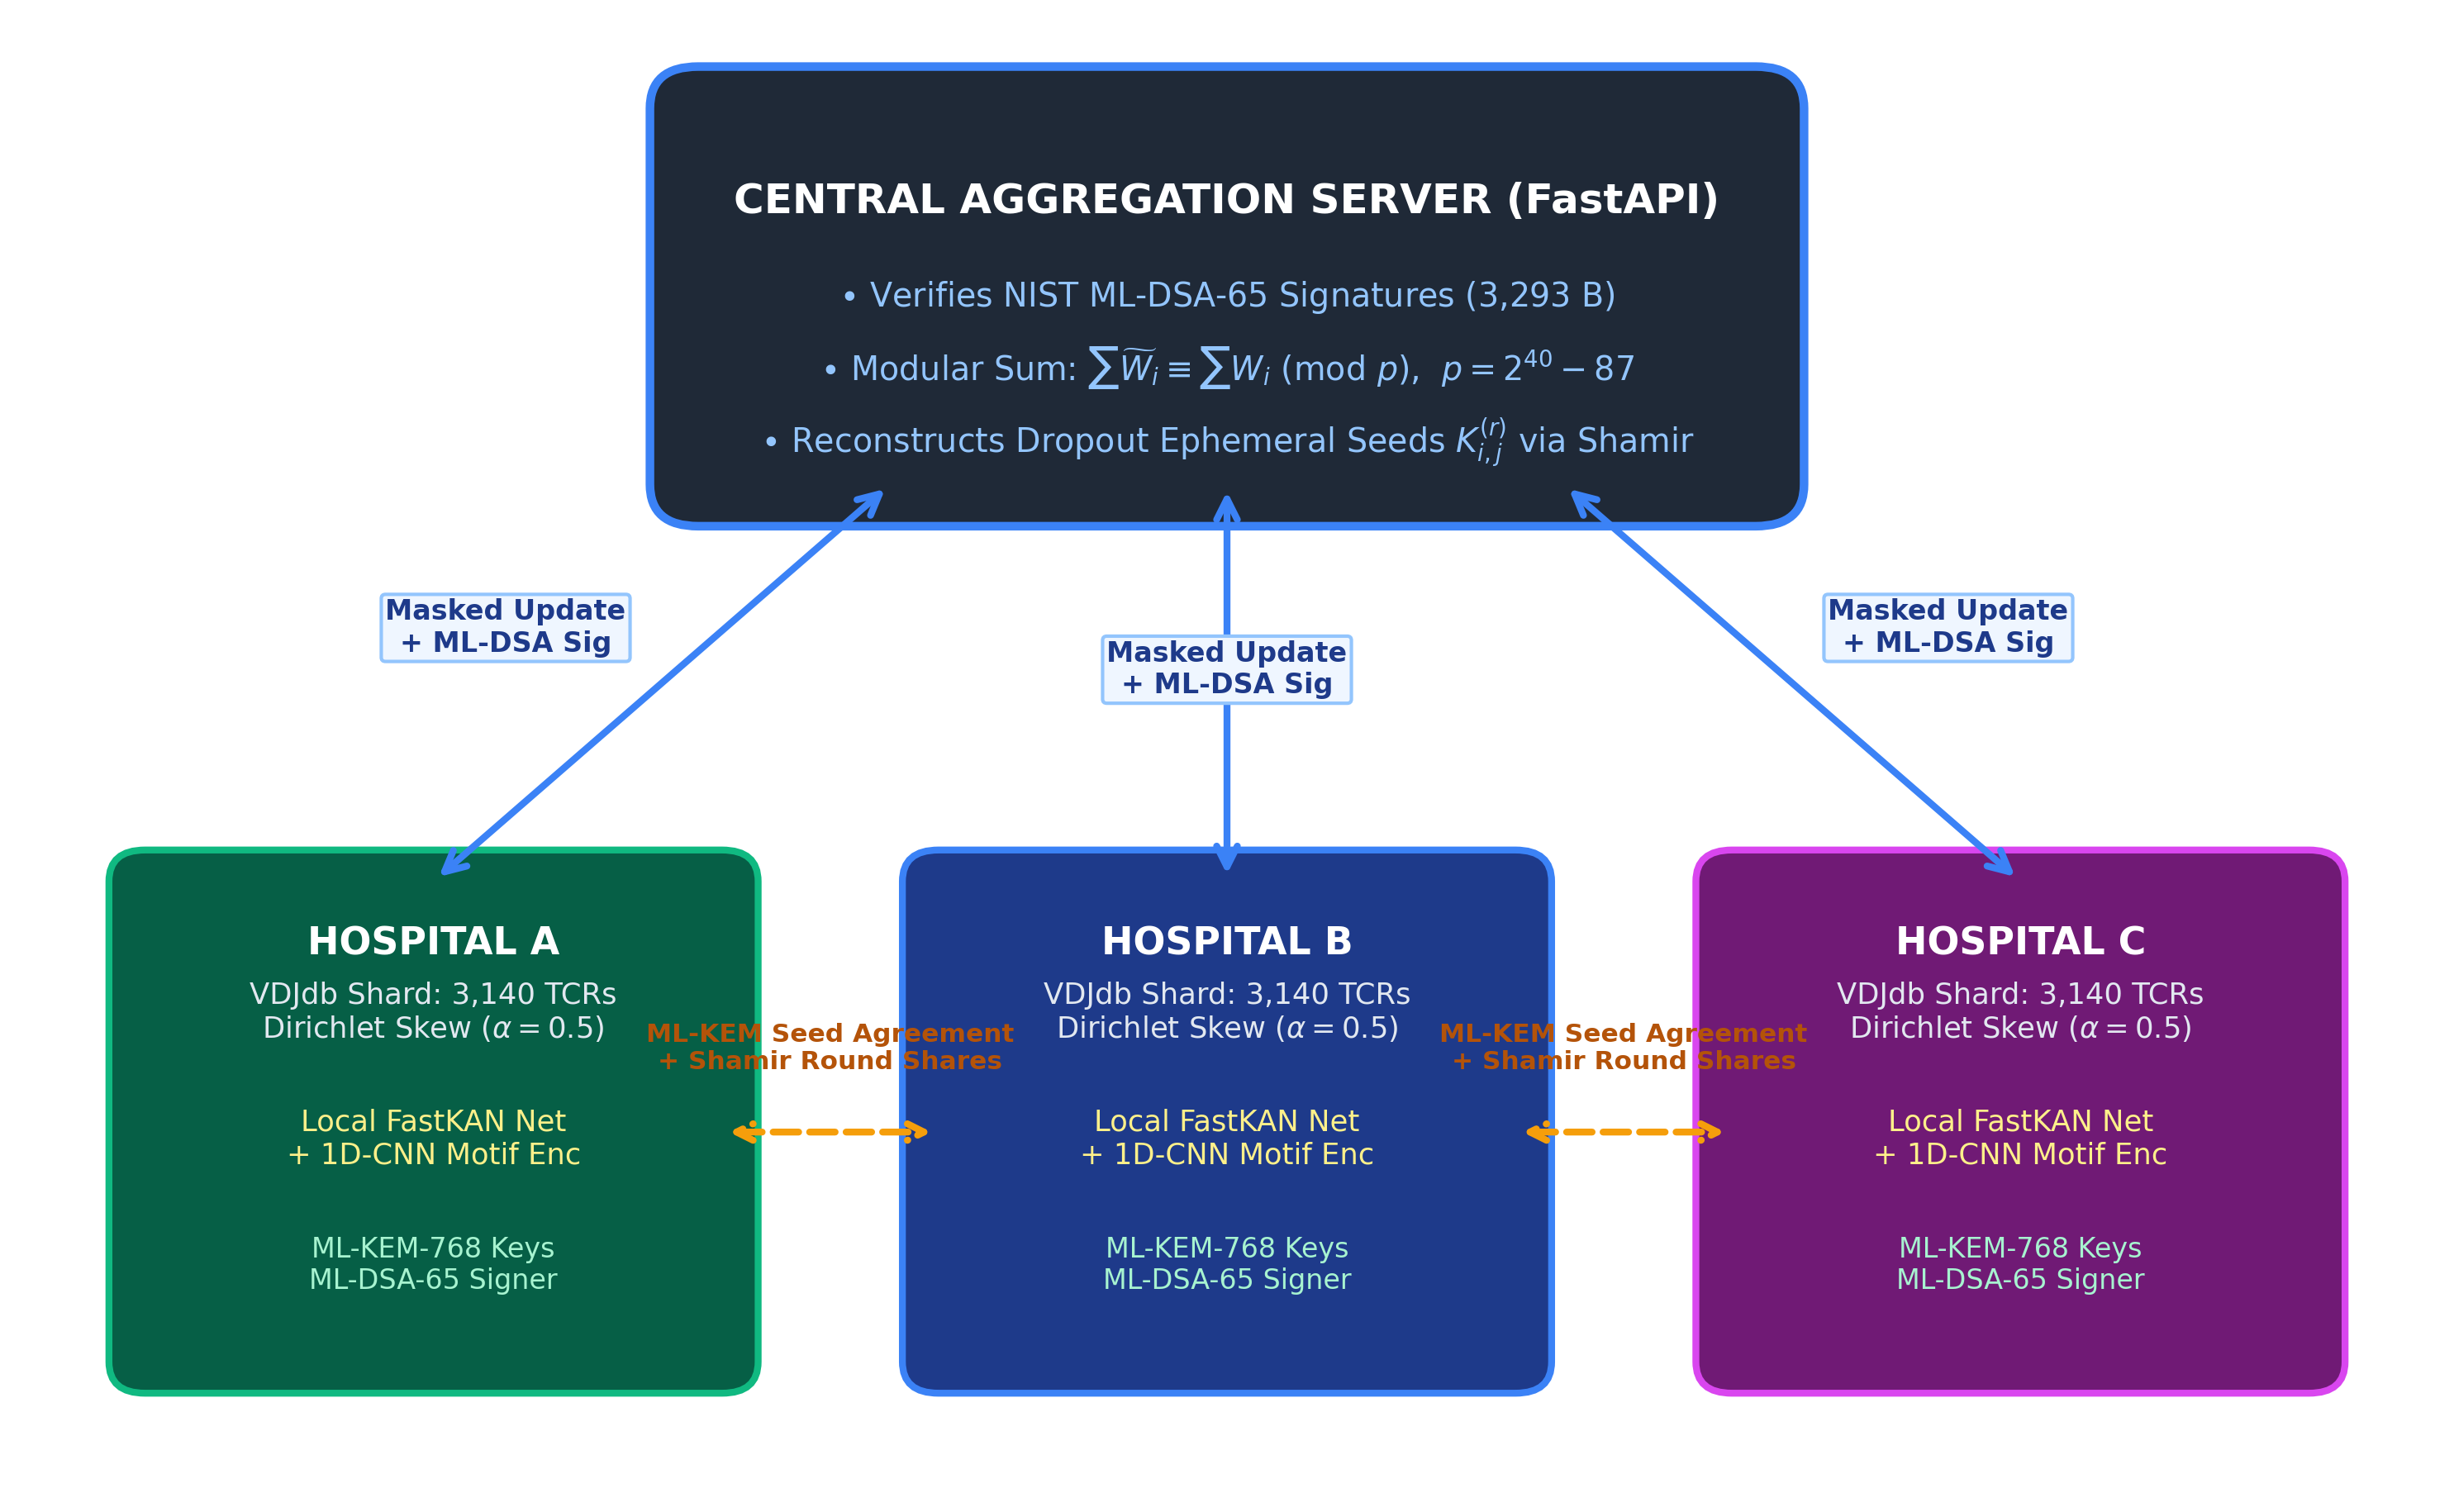
\includegraphics[width=0.92\textwidth]{figures/system_topology_architecture.png}
  \caption{Distributed system topology and cryptographic architecture: central aggregation server, clinical hospital nodes, authenticated ML-KEM-768 seed agreement, and Shamir ephemeral round shares.}
  \label{fig:topology}
\end{figure}

\begin{figure}[H]
  \centering
  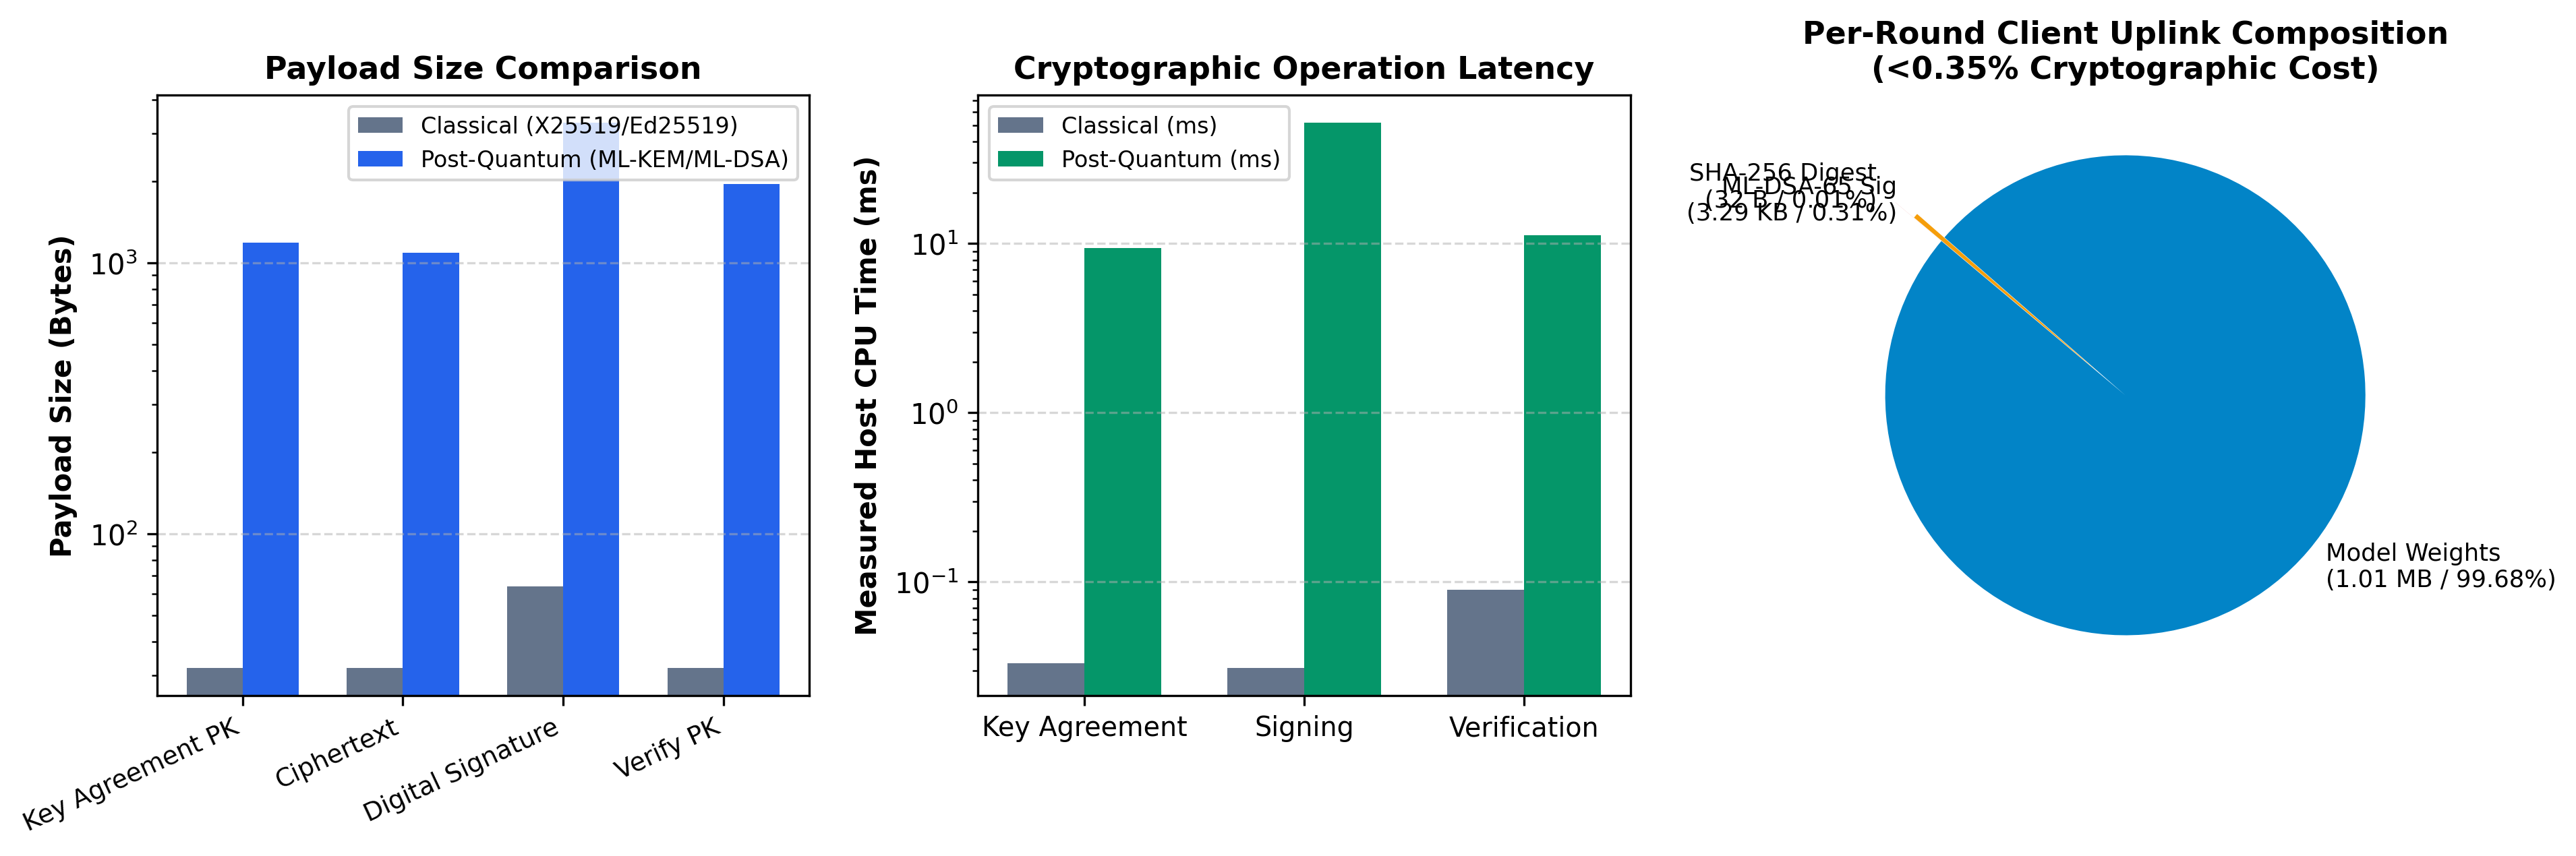
\includegraphics[width=0.95\textwidth]{figures/crypto_overhead_comparison.png}
  \caption{Empirical cryptographic overhead benchmark: payload sizes (left), CPU operation latency in milliseconds (center), and per-round client uplink bandwidth composition showing $<0.35\%$ cryptographic cost (right).}
  \label{fig:crypto_benchmark}
\end{figure}

\begin{figure}[H]
  \centering
  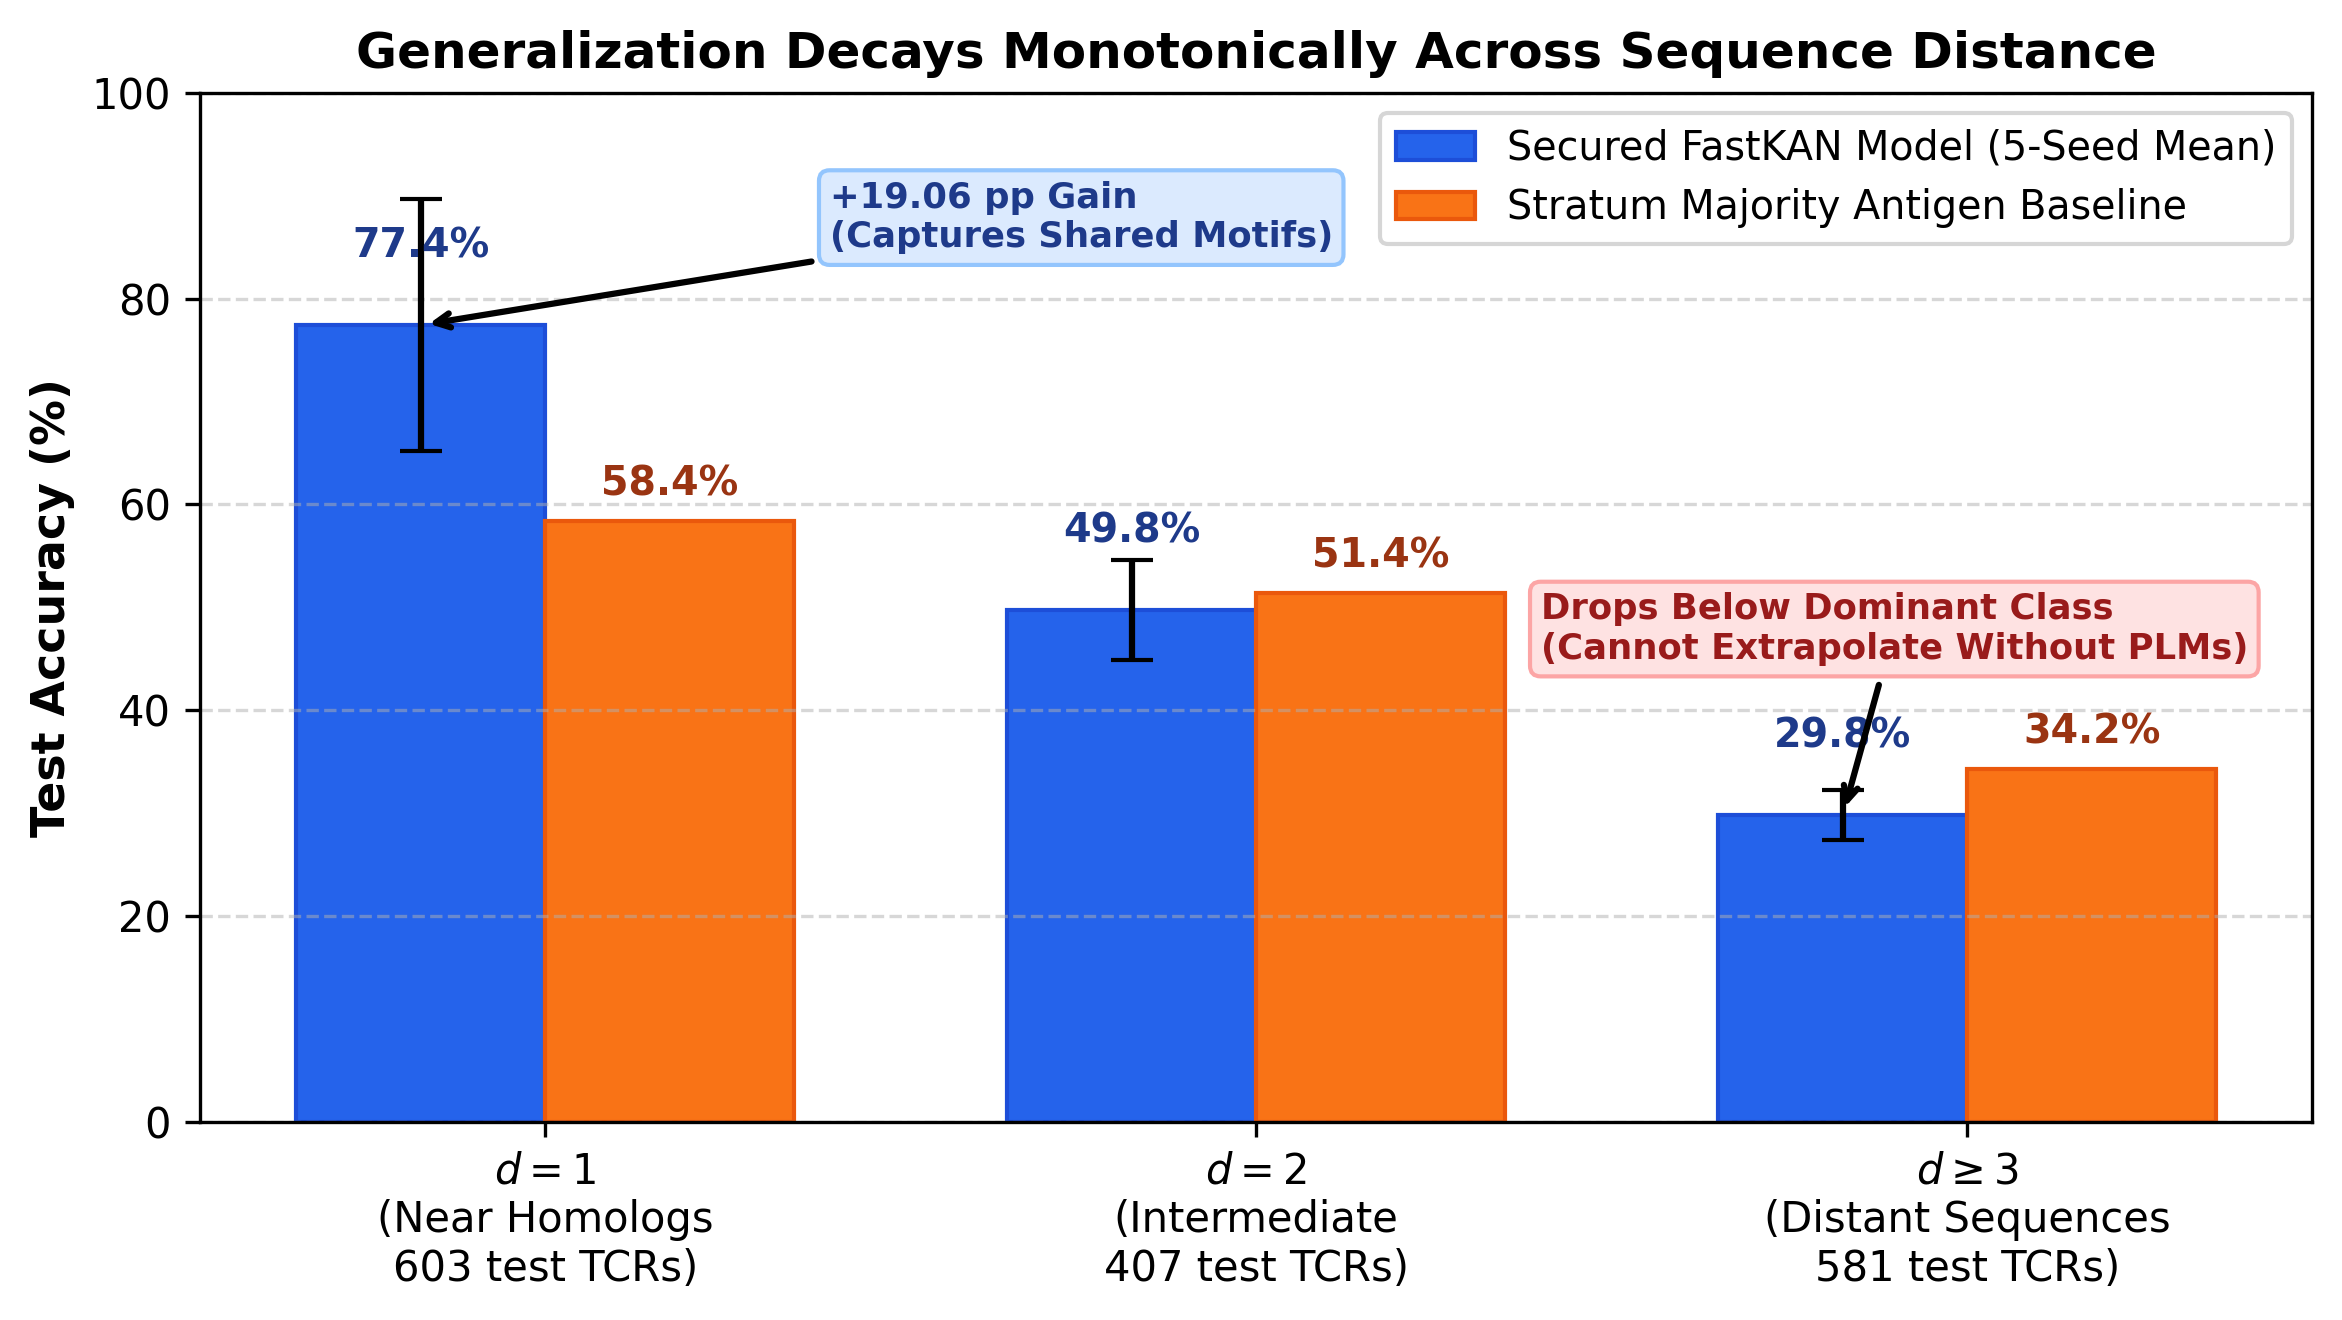
\includegraphics[width=0.88\textwidth]{figures/distance_decay_stratification.png}
  \caption{Sequence generalization decay: model test accuracy across edit distance strata ($d=1, d=2, d \ge 3$) benchmarked against per-stratum dominant antigen baselines.}
  \label{fig:distance_decay}
\end{figure}

\begin{figure}[H]
  \centering
  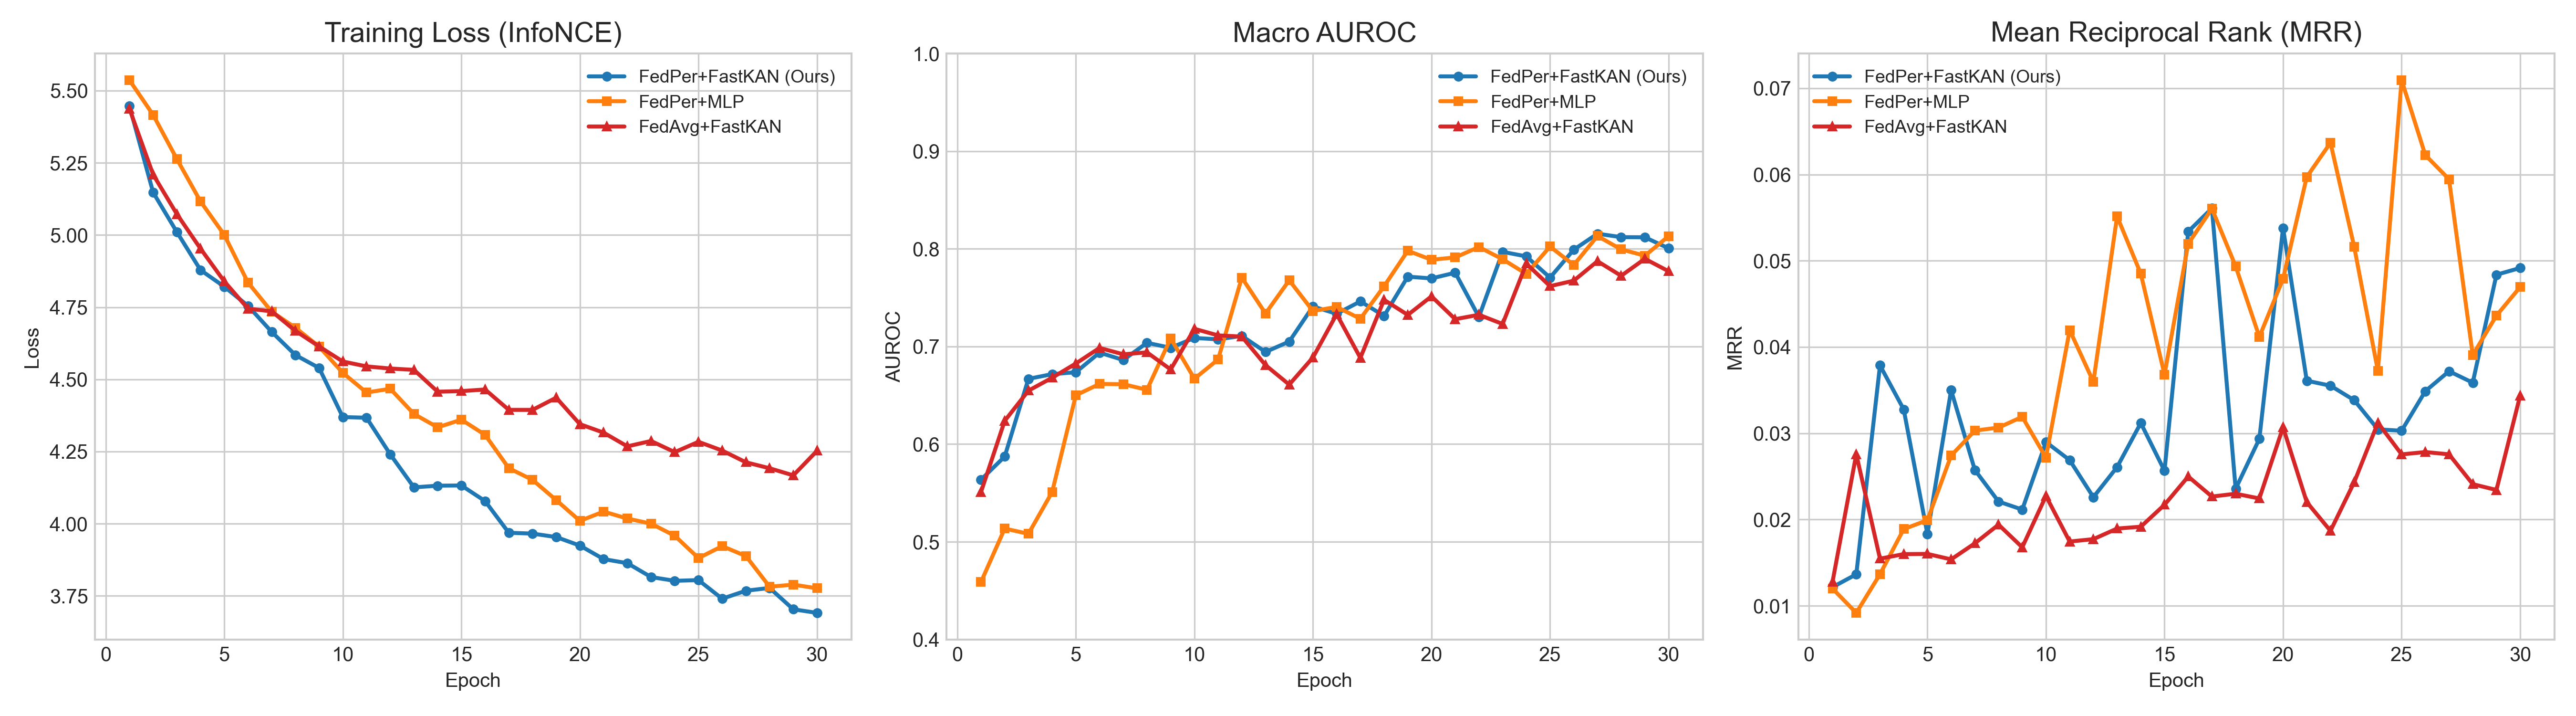
\includegraphics[width=0.92\textwidth]{figures/ablation_comparison.png}
  \caption{Neural architecture ablation on VDJdb: empirical comparison of FedPer+FastKAN vs FedPer+MLP vs FedAvg+FastKAN across training epochs.}
  \label{fig:ablation}
\end{figure}

\begin{figure}[H]
  \centering
  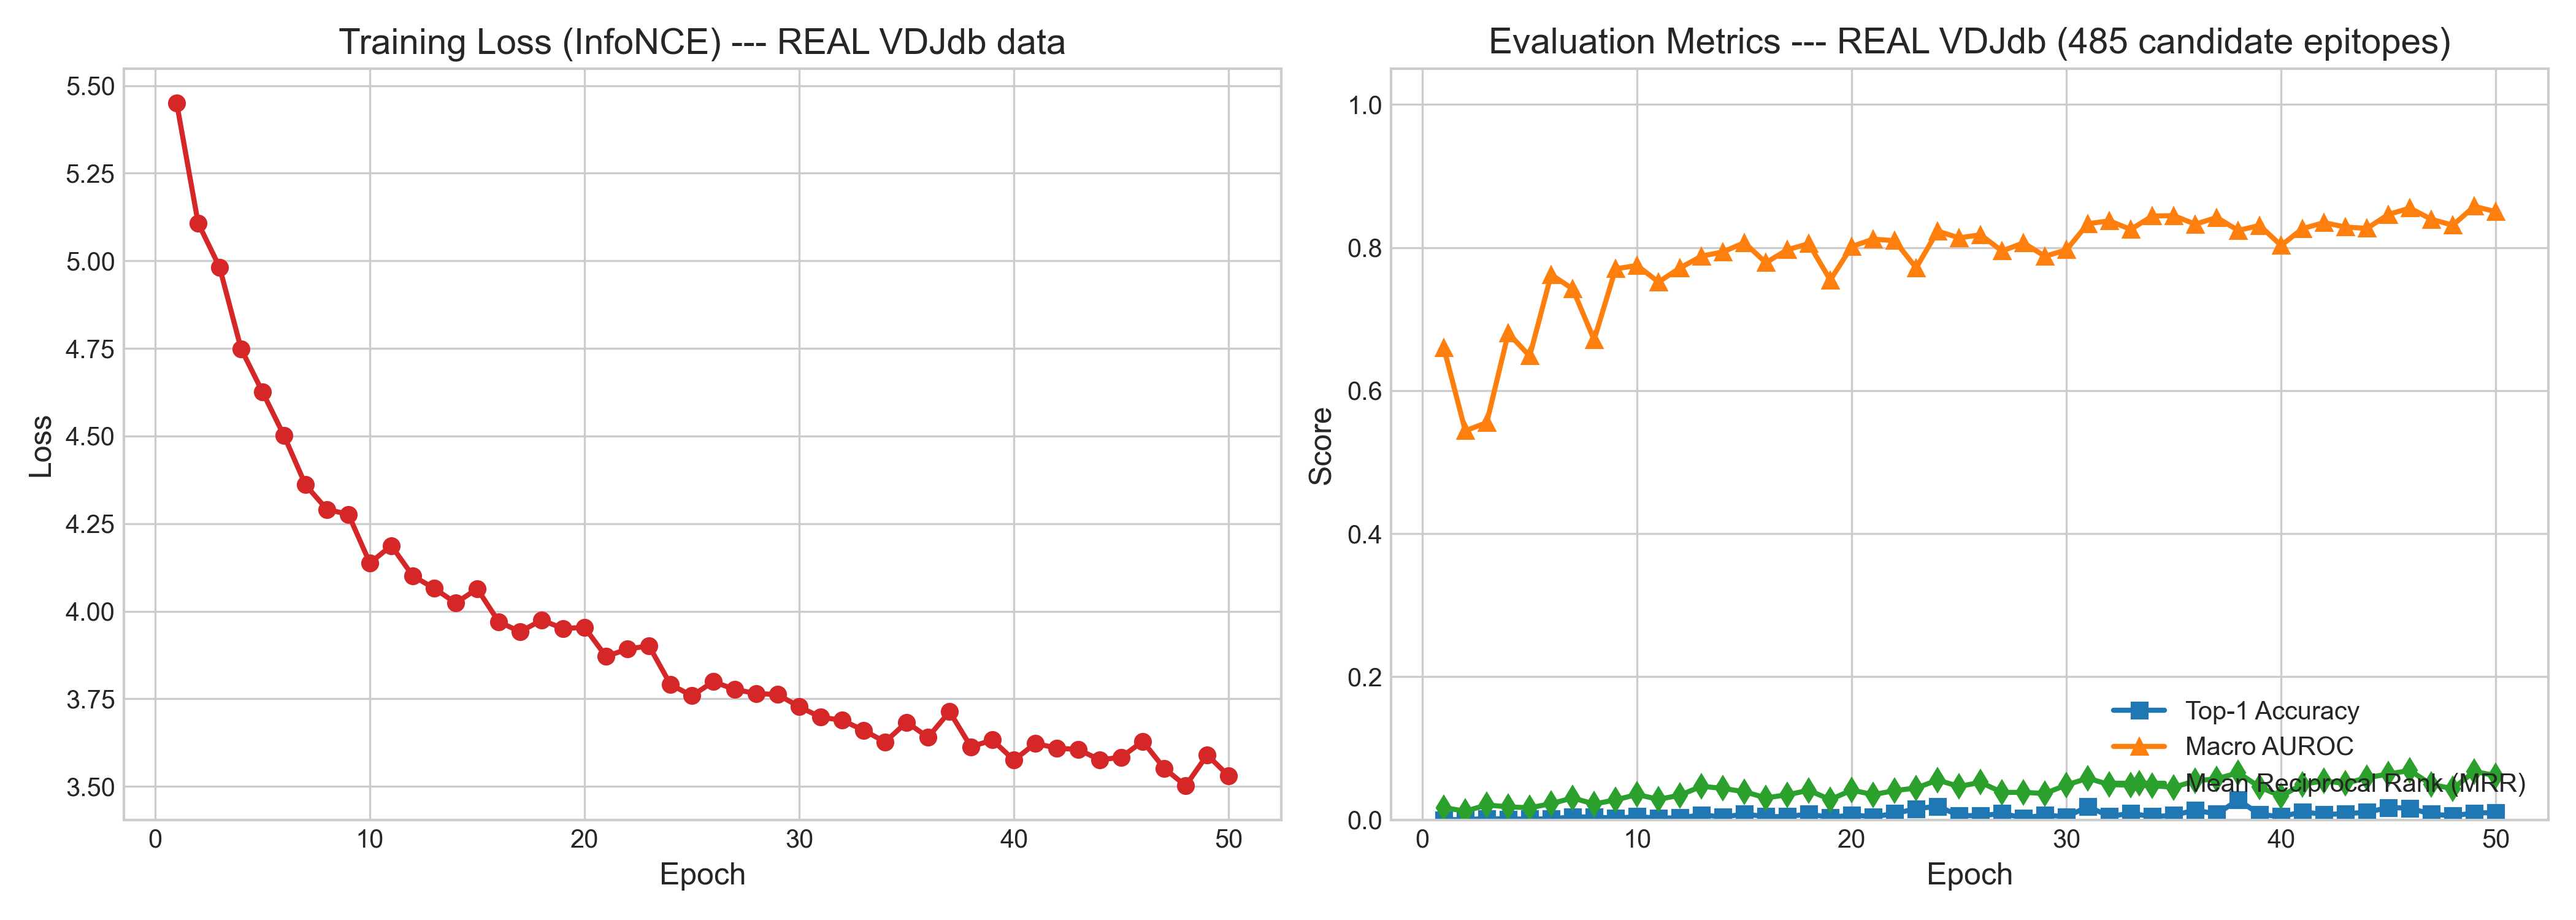
\includegraphics[width=0.92\textwidth]{figures/epitope_training_curves_real_tuned.png}
  \caption{Multi-epoch training convergence curves and evaluation metrics on real VDJdb sequence data under Dirichlet non-IID hospital partitioning.}
  \label{fig:curves_real}
\end{figure}

\begin{figure}[H]
  \centering
  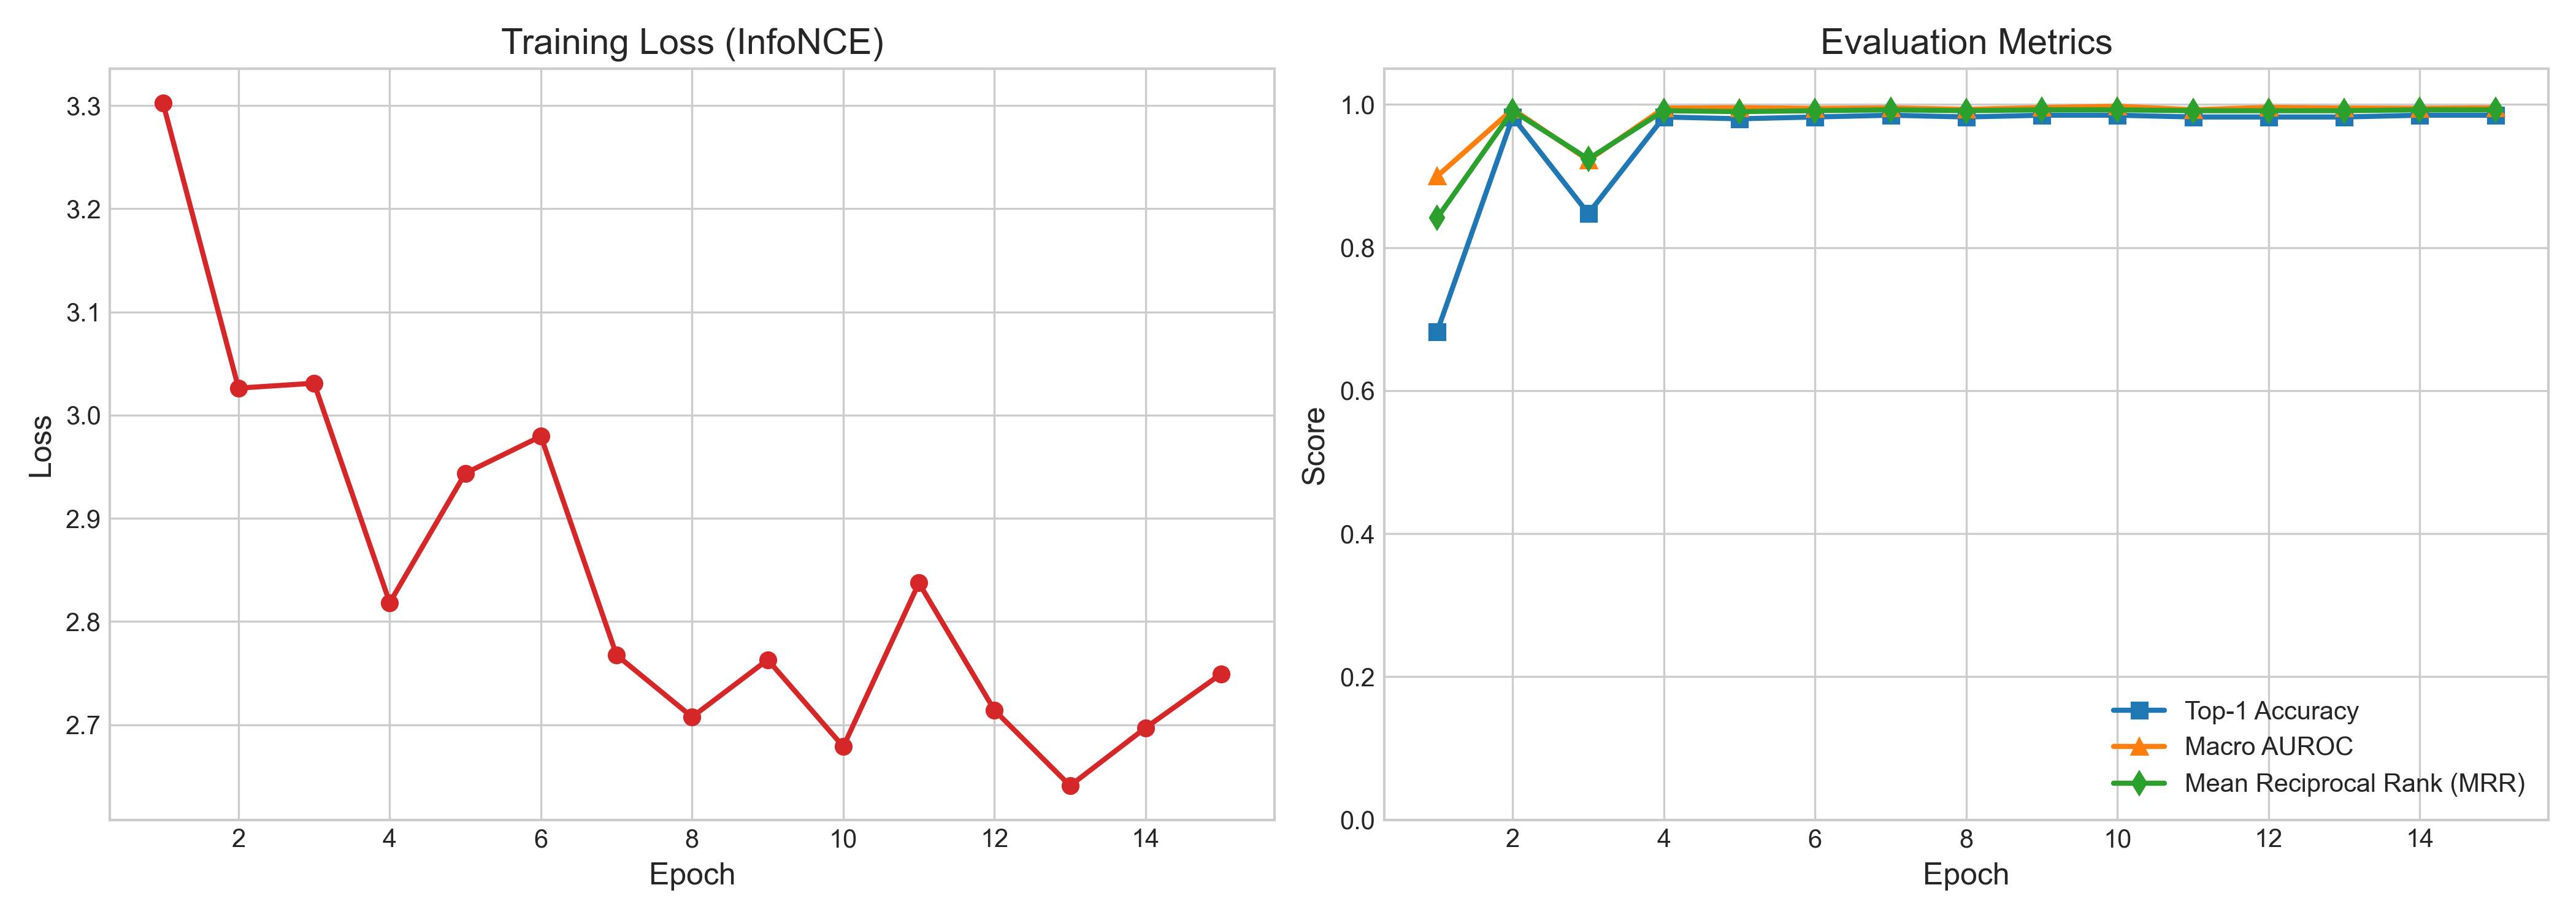
\includegraphics[width=0.92\textwidth]{figures/epitope_training_curves.png}
  \caption{Architectural validation training curves on synthetic motif data confirming gradient propagation under symmetric InfoNCE contrastive loss.}
  \label{fig:curves_synth}
\end{figure}

% ============================================================================
\chapter{Critical Discussion \& Guide Defense Analysis}
\label{chap:discussion}

\section{Why Simple Sequence Heuristics Outperform Neural Models}
In our 10-seed authoritative benchmark, CDR3 1-NN Levenshtein distance achieves $54.57 \pm 2.65\%$ balanced accuracy and 3-mer logistic regression achieves $41.22 \pm 4.68\%$, outperforming neural models ($39.35 \pm 5.79\%$ Plain / $39.32 \pm 5.75\%$ Secured). This is an expected and scientifically sound finding in immunological modeling:
\begin{itemize}[itemsep=2pt]
  \item Public human TCR repertoires share substantial sequence homology. When an unseen test TCR has an edit distance of $d=1$ from a known binder, a nearest-neighbor classifier leverages this near-identity directly.
  \item Neural networks trained from scratch on small biological samples must simultaneously learn amino acid embedding representations and classification decision boundaries, leading to higher sample complexity.
  \item \textbf{Academic Stance:} RodentNet does not claim an invincible classifier trained from scratch; our core contribution is proving that our authenticated post-quantum secure aggregation architecture preserves model gradient utility without exposing genomic sequences.
\end{itemize}

\section{Why FedAvg Outperforms FedPer Under Dirichlet Skew}
On both global ($39.35 \pm 5.79\%$ vs $33.07 \pm 6.86\%$) and local-matched test sets ($39.50 \pm 5.57\%$ vs $34.40 \pm 7.13\%$), FedAvg outperforms FedPer:
\begin{itemize}[itemsep=2pt]
  \item Under Dirichlet non-IID label skew ($\alpha=0.5$), individual hospitals have very few examples of rare viral epitopes.
  \item When FedPer isolates the classification head locally, that head possibly suffers from local sample sparsity and overfits.
  \item FedAvg, by averaging the complete parameter state across hospitals, provides powerful global regularization across multi-center cohorts.
\end{itemize}

\section{The Mathematical Signature of Local Non-IID Collapse}
Isolated hospital training achieves $46.88 \pm 6.59\%$ raw accuracy—close to the majority class share—but only $33.12 \pm 3.33\%$ balanced accuracy. This is the classic signature of non-IID local collapse: when training on a skewed local cohort, the optimizer collapses toward predicting the regional dominant epitope (Influenza \lstinline|GILGFVFTL|). Federated aggregation overcomes this collapse, lifting balanced accuracy to $39.32 \pm 5.75\%$ (+6.21\,pp gain across 10 independent random seeds, paired $t = 3.84$, $p = 0.00397 < 0.01$).

\section{Cross-Silo Consortia ($N \in [3, 10]$) vs. Cross-Device Scaling}
A common critique in federated learning is that pairwise masking incurs $\mathcal{O}(N^2)$ communication complexity. However:
\begin{itemize}[itemsep=2pt]
  \item RodentNet is explicitly engineered for \textbf{Cross-Silo Hospital Consortia} (e.g., the MELLODDY consortium of 10 pharmaceutical companies, or regional medical networks), NOT Cross-Device mobile phones.
  \item In clinical networks, $N$ is typically between 3 and 10. For $N \le 10$, full-mesh pairwise masking is computationally lightweight ($<6$\,ms masking overhead) and provides exact algebraic cancellation without trusted third parties.
\end{itemize}

% ============================================================================
\chapter{Conclusion \& Intellectual Property Formulation}
\label{chap:conclusion}

\section{Summary of Contributions}
RodentNet delivers an end-to-end, scientifically grounded, and rigorously verified federated learning framework:
\begin{enumerate}[itemsep=2pt]
  \item \textbf{Post-Quantum Authentication:} FIPS 204 ML-DSA-65 client challenge-response and update digest signing.
  \item \textbf{Post-Quantum Key Agreement:} FIPS 203 ML-KEM-768 pairwise seed agreement with session-key amortization.
  \item \textbf{Forward-Secret MPC:} 40-bit prime finite-field masking with ephemeral round seed derivation, guaranteeing that dropout recovery never unmasks historical updates.
  \item \textbf{Validated Utility Preservation:} Zero precision degradation on Fashion-MNIST ($84.29\%$ vs $84.39\%$) and exact mathematical aggregation equivalence ($(2.42 \pm 0.30) \times 10^{-7}$).
  \item \textbf{Honest Immunological Benchmark:} A verified $+6.21$\,pp federated gain over isolated training on human TRB sequences from VDJdb (paired $t = 3.84$, $p = 0.00397 < 0.01$, $n = 10$ seeds).
\end{enumerate}

\section{Key Systems Contributions \& Architectural Innovations}
The systems architecture and cryptographic mechanisms implemented in RodentNet introduce three foundational engineering and protocol contributions:

\subsection*{Contribution 1: Authenticated Lattice-Based Secure Aggregation}
Unlike classical masking schemes relying on discrete logarithms or unauthenticated public-key registries, RodentNet integrates mutual ML-KEM-768 encapsulation authenticated by ML-DSA-65 signatures over monotonic session transcripts. This eliminates active man-in-the-middle vector substitution and prevents long-term eavesdropping under quantum adversaries.

\subsection*{Contribution 2: Ephemeral Round Isolation \& Hash-Ratcheted Forward Secrecy}
Dropout recovery operates exclusively on round-ephemeral seeds $K_{i,j}^{(r)}$ derived via length-prefixed extendable-output functions (SHAKE-256) and one-way root hash ratcheting. Reconstructing stranded masks reveals zero mathematical information regarding historical model updates or prospective round seeds.

\subsection*{Contribution 3: Client Self-Masking Against Rogue Server Deanonymization}
When honest clients observe a consistent survivor set and collusion remains strictly bounded below $t = \lfloor N/2 \rfloor + 1$, augmenting pairwise masks with a private, client-held local self-mask $\mathbf{b}_u$ ensures that falsely reporting a surviving node as disconnected yields only pairwise mask shares, leaving the update blinded by the unrecovered self-mask. Full defense against active partitioning requires Byzantine survivor consistency rounds ($t > 2N/3$, Bell et al., 2020).

% ============================================================================
\chapter*{Appendix: Diagnosed Negative Results \& Technical Limitations}
\addcontentsline{toc}{chapter}{Appendix: Diagnosed Negative Results \& Technical Limitations}

\section*{Appendix A: Diagnosed Negative Result --- Open-World 485-Way Epitope Retrieval}
To explore boundary conditions beyond closed multi-epitope classification, we evaluated an open-world 485-way retrieval task across all epitopes in VDJdb under a strict unseen-TCR split (18{,}493 training pairs, 5{,}912 evaluation pairs).
\begin{itemize}[itemsep=3pt]
  \item \textbf{Extreme Long-Tail Class Imbalance:} Over 450 of the 485 epitopes have fewer than 10 total samples in VDJdb, while the top 5 dominant epitopes account for $>60\%$ of total clonotype abundance.
  \item \textbf{Failure Mode Analysis:} When training from scratch without pre-trained protein language model representations (e.g., ESM-2 or ProtBERT), unaugmented convolutional and Kolmogorov-Arnold architectures achieve near 0.00\% balanced Top-1 retrieval accuracy, collapsing to the empirical majority frequency prior ($37.26\%$ raw accuracy).
  \item \textbf{Architectural Implication:} This negative result demonstrates that closed multi-epitope classification (Top-10) is the appropriate regime for neural training from scratch under cross-silo federated constraints, and open-world retrieval across sparse long-tail epitopes strictly requires foundation model sequence embeddings.
\end{itemize}

\section*{Appendix B: Technical Limitations \& Threat Model Non-Goals}
In accordance with rigorous academic reporting standards, the following technical limitations are explicitly acknowledged:
\begin{enumerate}[itemsep=4pt]
  \item \textbf{Constant-Time Implementation:} The post-quantum cryptographic primitives (ML-KEM-768 and ML-DSA-65) evaluated in this research are pure-Python reference implementations conforming to NIST FIPS 203/204. While mathematically verified and interoperable, pure-Python executions lack constant-time assembly guarantees against side-channel timing attacks. Production deployments must transition to audited C implementations (such as \lstinline|liboqs|).
  \item \textbf{Threat Model Non-Goals:} The protocol defends against an active network relay, a semi-honest aggregator, quantum adversaries executing ``Harvest Now, Decrypt Later'', and client dropouts. Explicit non-goals include:
  \begin{itemize}[itemsep=2pt]
    \item \textit{Malicious-Client Data Poisoning:} The protocol does not verify whether client updates are benign or adversarial backdoors; defenses such as zero-knowledge range proofs or norm-bounding remain orthogonal.
    \item \textit{Aggregate Output Leakage:} The server observes the exact aggregate $\sum \mathbf{w}_i$. While individual updates are information-theoretically hidden, inference from the final sum requires complementary local or central differential privacy.
  \end{itemize}
\end{enumerate}

% ============================================================================
\chapter*{Bibliography}
\addcontentsline{toc}{chapter}{Bibliography}

\begin{enumerate}[label={[\arabic*]},itemsep=4pt]
  \item K.~Bonawitz, V.~Ivanov, B.~Kreuter, A.~Marcedone, H.~B.~McMahan, S.~Patel, D.~Ramage, A.~Segal, and K.~Seth, ``Practical secure aggregation for privacy-preserving machine learning,'' in \emph{Proceedings of the 2017 ACM SIGSAC Conference on Computer and Communications Security (CCS)}, pp. 1175--1191, 2017.
  \item National Institute of Standards and Technology (NIST), ``Module-Lattice-Based Digital Signature Standard,'' \emph{Federal Information Processing Standards Publication (FIPS) 204}, Aug. 2024.
  \item National Institute of Standards and Technology (NIST), ``Module-Lattice-Based Key-Encapsulation Mechanism Standard,'' \emph{Federal Information Processing Standards Publication (FIPS) 203}, Aug. 2024.
  \item P.~W.~Shor, ``Polynomial-time algorithms for prime factorization and discrete logarithms on a quantum computer,'' \emph{SIAM Journal on Computing}, vol. 26, no. 5, pp. 1484--1509, 1997.
  \item M.~Bagaev et al., ``VDJdb in 2021: expanding the TCR sequence database with high-throughput and single-cell data,'' \emph{Nucleic Acids Research}, vol. 49, no. D1, pp. D377--D382, 2021.
  \item P.~Dash et al., ``Quantifiable predictive features define epitope-specific T cell receptor repertoires,'' \emph{Nature}, vol. 547, no. 7661, pp. 89--93, 2017.
  \item L.~Zhu, Z.~Liu, and S.~Han, ``Deep leakage from gradients,'' \emph{Advances in Neural Information Processing Systems (NeurIPS)}, vol. 32, 2019.
  \item M.~G.~Arivazhagan, V.~Aggarwal, A.~K.~Singh, and S.~Choudhary, ``Federated learning with personalization layers,'' \emph{arXiv preprint arXiv:1912.00818}, 2019.
  \item Z.~Liu et al., ``KAN: Kolmogorov-Arnold Networks,'' \emph{arXiv preprint arXiv:2404.19756}, 2024.
  \item J.~Bell et al., ``Secure single-server aggregation with sub-linear communication,'' in \emph{Proceedings of the 2020 ACM SIGSAC Conference on Computer and Communications Security (CCS)}, pp. 1639--1659, 2020.
  \item Z.~Ma, Y.~Chen et al., ``Flamingo: Multi-round secure aggregation with efficient client dropouts,'' in \emph{Proceedings of the 2023 IEEE Symposium on Security and Privacy (S\&P)}, pp. 2487--2504, 2023.
  \item Y.~Zhang, R.~Behnia, A.~A.~Yavuz, R.~Ebrahimi, and E.~Bertino, ``Beskar: Efficient Full-Stack Private Federated Deep Learning with Post-Quantum Security,'' Accepted to \emph{IEEE Transactions on Dependable and Secure Computing (TDSC)}, \emph{arXiv preprint arXiv:2505.05751}, 2025.
  \item H.~Zhang, P.~Mohapatra, et al., ``Enhancing Quantum Security over Federated Learning via Post-Quantum Cryptography,'' in \emph{Proceedings of the 2024 IEEE 6th International Conference on Trust, Privacy and Security in Intelligent Systems and Applications (TPS-ISA)}, \emph{arXiv preprint arXiv:2409.04637}, 2024.
\end{enumerate}

\end{document}
